\documentclass[12pt]{article}
\usepackage[margin=1in]{geometry}
\usepackage{amsmath,amssymb}
\usepackage{booktabs,threeparttable,multirow,makecell,float,graphicx,caption}
\usepackage[normalem]{ulem}
\usepackage{setspace}
\usepackage[hidelinks]{hyperref}
\usepackage{natbib}
\bibliographystyle{aer}
\onehalfspacing

\title{Who Gets the Whistle? Refereeing Decisions and FC Barcelona in European Football, 2001--2026}
\author{Hussain Hadah}
\date{\today}

\begin{document}
\maketitle

\begin{abstract}
\noindent Do some football clubs receive systematically more favorable refereeing decisions? I assemble match-level data on fouls, cards, penalties, and stoppage time for the five largest European leagues and the UEFA Champions League from 2001/02 to 2025/26, about 48,500 matches. I ask where FC Barcelona sits relative to every other club before and after 2018, the year in which the club's reported payments to the vice-president of Spain's referees' committee ended. Raw comparisons strongly favor Barcelona, but they largely reflect its possession-dominant style. Conditional on opponent, home status, pre-match odds, and possession, Barcelona receives 0.17--0.23 fewer yellow cards per match than the average club. Conditional on fouls called, it receives no fewer cards, and its penalty treatment is unremarkable: it ranks 93rd of 150 clubs on net penalties. Normalizing fouls by possession reverses the sign of its foul advantage. Barcelona's net card advantage in La Liga declines after 2017/18 relative to Real Madrid (by 0.57 cards per match), but the timing tracks its sporting decline and Messi's departure at least as closely as the end of the payments. The clearest favoritism is in stoppage time: referees add about 0.7 more minutes when Barcelona trails than when it leads. Real Madrid receives the same advantage, suggesting status-based social pressure rather than a club-specific arrangement.


\medskip
\noindent \textbf{JEL Codes:} D73, L83, Z20, Z28. \quad
\textbf{Keywords:} referee bias, favoritism, corruption, social pressure, football.
\end{abstract}

\newpage
\section{Introduction}\label{sec:intro}

Referees are agents whose decisions are subjective, consequential, and observed by large and partisan audiences. A large literature documents that these decisions respond to social pressure, most prominently in the form of home bias in stoppage time, cards, and penalties \citep{sutter2004favoritism, garicano2005favoritism, boyko2007referee, dohmen2008influence, rickman2008favouritism, scoppa2008subjective, buraimo2010twelfth}. Natural experiments that removed crowds, from stadium closures in Italy to the Covid-19 ``ghost games,'' show that much of this bias disappears without spectators \citep{pettersson2010behavior, endrich2020home, bryson2021causal, reade2022eliminating}. Explicit corruption has also been documented: the 2006 \textit{Calciopoli} scandal in Italy revealed referee designations steered toward favored clubs \citep{boeri2011match}.

Much less is known about whether particular \emph{clubs}, as opposed to home teams, receive favorable treatment, and how large such an advantage is relative to every other club. The question is pressing in Spain. In 2023, prosecutors alleged that FC Barcelona had paid about XX [verify: reported as roughly \texteuro 7 million] between 2001 and 2018 to companies owned by José María Enríquez Negreira, then vice-president of the Comité Técnico de Árbitros (CTA), the body that oversees Spanish referees.\footnote{XX: Add the source for the prosecutor's complaint (March 2023) and the reported amounts. Whether any refereeing decision was affected is the subject of ongoing legal proceedings; this paper makes no claim about the legal case.} Whether those payments bought anything on the pitch is ultimately an empirical question about refereeing decisions.

In this paper, I ask three questions. First, do referees in the top-5 European leagues make systematically more favorable decisions for some clubs than for others? Second, where does Barcelona sit in that distribution, compared with Real Madrid, the other elite clubs, and every other club? Third, is Barcelona treated differently by Spanish referees than by UEFA referees, and did that difference change after 2017/18?

To answer these questions, I assemble match-level data on fouls, cards, penalties, possession, and stoppage time for about 48,500 matches in the Premier League, La Liga, Serie A, the Bundesliga, Ligue 1, and the Champions League between 2001/02 and 2025/26. I link these data to pre-match bookmaker odds. I estimate club-specific decision gaps conditional on opponent, home status, league-season, and pre-match win probability. I place Barcelona's estimate in the distribution of estimates for all 144 clubs with at least 150 matches, which serves as a permutation-style benchmark. To separate club-level playing style from referee behavior, I exploit the fact that Barcelona's style travels to the Champions League while its Spanish referees do not. I also normalize fouls by possession, which measures a side's exposure to being fouled.

Preview of findings. Raw comparisons strongly favor Barcelona, but they mostly reflect its possession-dominant style. Conditional on fouls called, Barcelona's players are no less likely to be booked, and its opponents are no more likely. On penalties, Barcelona ranks 93rd of 150 clubs. Normalizing fouls by possession reverses the sign of its foul advantage. Barcelona's net yellow-card advantage in La Liga does decline after 2017/18 relative to Real Madrid, by 0.57 cards per match. That decline coincides with Barcelona's sporting and financial crisis, and its net-foul advantage breaks only in 2021/22, the season Messi left. The clearest evidence of favoritism is in stoppage time: referees add about 0.7 more minutes when Barcelona trails by a goal than when it leads, but Real Madrid enjoys exactly the same advantage.

This paper contributes to the literature on favoritism and social pressure in refereeing by moving from home bias to club-specific bias, and by benchmarking a single club against the full cross-section of clubs. It also contributes to the literature on corruption in sports \citep{boeri2011match} by showing how far observable decisions can and cannot speak to an alleged corrupt relationship.

The rest of the paper is organized as follows. Section \ref{sec:data} describes the data. Section \ref{sec:strategy} presents the empirical strategy. Section \ref{sec:results} reports the results. Section \ref{sec:conclusion} concludes.

\section{Data}\label{sec:data}

I assemble match-level refereeing data for the five largest European leagues (the English Premier League, Spain's La Liga, Italy's Serie A, Germany's Bundesliga, and France's Ligue 1) and the UEFA Champions League from 2001/02 to 2025/26. The data combine two sources.

The first is ESPN's public match-summary interface, which reports for each match the teams, the score, fouls, yellow and red cards, possession, shots, attendance, the referee, and a log of key events with the match clock.\footnote{The interface is \texttt{site.api.espn.com/apis/site/v2/sports/soccer}. ESPN team identifiers are consistent across competitions, so Barcelona's La Liga and Champions League matches link without a name crosswalk.} From the event log, I count penalties awarded to each side (scored, missed, saved, or striking the woodwork, excluding shoot-outs), the score at 90 minutes, and first- and second-half stoppage time. The second source is football-data.co.uk, which provides pre-match bookmaker odds for every domestic match and an independent record of fouls and cards. I convert odds into win probabilities normalized for the bookmaker margin. Where both sources report fouls and cards, they agree exactly in 92--98 percent of matches (correlation above 0.97), and I fill gaps in one source with the other. For the Champions League, where odds are unavailable, I measure pre-match strength with Elo ratings computed from all results in the data.

I restrict the analysis to completed seasons and drop Champions League qualifying rounds. Fouls and cards are reliably recorded from 2005/06 onward; penalties from 2001/02 in league-seasons whose event logs are complete.\footnote{I treat a league-season's penalty record as incomplete when it shows fewer than 0.15 penalties per match, well below the 0.25--0.35 typical of these leagues.} The unit of analysis is the team-match: each match enters twice, once from each side's perspective. Decisions ``against'' team $i$ are the fouls, cards, and penalties called on $i$; decisions ``for'' $i$ are those called on its opponent. The analysis panel contains 96,956 team-matches (48,478 matches) involving 313 clubs; Barcelona contributes 950 La Liga and 263 Champions League matches.

Table \ref{tab:sumstats} reports per-match means for Barcelona, Real Madrid, the other La Liga clubs, the twelve other elite clubs, and all remaining clubs, separately for domestic leagues and the Champions League. I discuss these means in Section \ref{sec:results}.

\section{Empirical Strategy}\label{sec:strategy}

\subsection{Club-specific refereeing gaps}

I begin by estimating how refereeing decisions for Barcelona differ from those for the average club in the same league-season, holding fixed the circumstances of the match. Let $D_{imt}$ denote a refereeing decision (yellow cards, red cards, fouls called, penalties) against or in favor of team $i$ in match $m$ of season $t$. I estimate
\begin{equation}\label{eq:teamfe}
D_{imt} = \beta_1 \text{Barcelona}_i + \beta_2 \text{RealMadrid}_i + \beta_3 \text{Elite}_i + \delta\, \text{Home}_{im} + \mu_{o(im)} + \lambda_{\ell t} + \psi_{p(im)} + \varepsilon_{imt},
\end{equation}
where $\text{Elite}_i$ indicates the twelve other perennial Champions League clubs, $\mu_{o(im)}$ are opponent fixed effects, $\lambda_{\ell t}$ are league $\times$ season fixed effects, and $\psi_{p(im)}$ are fixed effects for ventiles of the pre-match win probability implied by bookmaker odds. The coefficient $\beta_1$ is the gap in decisions between Barcelona and an average non-elite club in the same league-season that faces the same opponent with the same pre-match chance of winning. The identifying assumption is that, conditional on these controls, Barcelona's matches generate the same rate of card-, foul-, and penalty-worthy events as the comparison clubs'. The main threat is playing style: a possession-dominant club commits fewer fouls and suffers more of them because it has the ball. I address this in three ways. First, I add fixed effects for 2.5-point possession bins and both teams' shots (Panel B of Table \ref{tab:teamfe}), recognizing that in-game variables may themselves respond to refereeing decisions. Second, I estimate the referee's severity conditional on fouls: yellow cards controlling for the number of fouls called. Third, I normalize fouls by possession and passes, the side's exposure (Table \ref{tab:exposure}).

\subsection{Barcelona in the cross-club distribution}

With a single club of interest, conventional cluster-robust inference is fragile. I therefore place Barcelona's estimate in the distribution of estimates for every club. For each net decision $\Delta D_{imt}$ (decisions in favor minus decisions against), I estimate
\begin{equation}\label{eq:ranks}
\Delta D_{imt} = \alpha_i + \mu_{o(im)} + \lambda_{\ell t} + \psi_{p(im)} + \delta\, \text{Home}_{im} + u_{imt},
\end{equation}
normalize the club fixed effects $\alpha_i$ to the match-weighted average club in each league, and report Barcelona's rank among all clubs with at least 150 matches. The share of clubs at least as favored as Barcelona is a permutation-style $p$-value.

\subsection{Spanish versus UEFA referees}

Barcelona's style, squad, and status travel with it to the Champions League, but its referees do not: UEFA never appoints a referee from a club's own federation. Among the clubs with at least 40 Champions League matches, I estimate
\begin{equation}\label{eq:ddd}
\begin{split}
D_{imt} = {} & \sum_{p \in \{\text{pre},\text{post}\}} \left[\beta_p\, \text{Barcelona}_i + \rho_p\, \text{RealMadrid}_i\right] \times \text{Domestic}_m \times \mathbb{1}[t \in p] \\
& + \theta_{i,p} + \kappa_{\ell(i), \text{Dom}, p} + \tau_{c(m) t} + \psi_{e(im)} + \delta\, \text{Home}_{im} + \varepsilon_{imt},
\end{split}
\end{equation}
where $\theta_{i,p}$ are club $\times$ period fixed effects, $\kappa_{\ell(i),\text{Dom},p}$ are home-league $\times$ domestic $\times$ period fixed effects, $\tau_{c(m)t}$ are competition $\times$ season fixed effects, and $\psi_{e(im)}$ are fixed effects for ventiles of the Elo expected score. The pre period is 2001/02--2017/18, the seasons covered by the reported payments to the vice-president of the CTA; the post period is 2018/19--2025/26. $\beta_p$ measures how much more favorably Spanish referees treat Barcelona than UEFA referees do, relative to the same gap for the other Spanish Champions League regulars. $\beta_{\text{post}} - \beta_{\text{pre}}$ is a triple difference. Its identifying assumption is that, absent a change in Barcelona's relationship with Spanish refereeing, Barcelona's domestic-versus-European gap would have evolved like that of the other regulars. The end of the payments coincides with the introduction of VAR in La Liga (2018/19) and in the Champions League knockout rounds (2018/19), which the competition $\times$ season fixed effects absorb if VAR affects clubs equally.

\subsection{Season-by-season gaps}

To trace the timing, I estimate the La Liga analogue of equation (\ref{eq:teamfe}) with season-specific Barcelona and Real Madrid indicators:
\begin{equation}\label{eq:eventstudy}
\begin{split}
\Delta D_{imt} = {} & \sum_{s} \beta_s\, \text{Barcelona}_i \mathbb{1}[t=s] + \sum_{s} \rho_s\, \text{RealMadrid}_i \mathbb{1}[t=s] \\
& + \delta\, \text{Home}_{im} + \lambda_t + \mu_{o(im)} + \psi_{p(im)} + \pi_{b(im)} + \varepsilon_{imt},
\end{split}
\end{equation}
where $\pi_{b(im)}$ are possession-bin fixed effects.

\subsection{Stoppage time}

Following \citet{garicano2005favoritism}, I test whether referees lengthen matches when a favored side trails and shorten them when it leads. For domestic matches whose score margin at 90 minutes is at most one goal,
\begin{equation}\label{eq:stoppage}
\begin{split}
\text{Stoppage}_m = {} & \sum_{g} \left[a_g \text{Leads}_{gm} + c_g \text{Trails}_{gm} + d_g \text{Tied}_{gm}\right] \\
& + b_L \text{HomeLeads}_m + b_T \text{HomeTrails}_m + X_m \pi + \lambda_{\ell t} + \varepsilon_m,
\end{split}
\end{equation}
where $g \in \{\text{Barcelona}, \text{Real Madrid}\}$ and $X_m$ contains second-half goals and total cards and penalties. Favoritism toward club $g$ implies $c_g - a_g > 0$.

\subsection{Real Madrid in the Champions League}

To study Real Madrid's treatment by UEFA referees, I estimate on the Champions League team-match panel
\begin{equation}\label{eq:rmucl}
\begin{split}
\Delta D_{imt} = {} & \sum_{s} \left[r_s\, \text{RealMadrid}_i + b_s\, \text{Barcelona}_i + e_s\, \text{Elite}_i\right] \mathbb{1}[t=s] \\
& + \delta\, \text{Home}_{im} + \lambda_t + \sigma_{g(m)} + \mu_{o(im)} + \psi_{e(im)} + \pi_{b(im)} + \varepsilon_{imt},
\end{split}
\end{equation}
where $\sigma_{g(m)}$ are stage fixed effects (group/league phase, knockout), $\psi_{e(im)}$ are Elo expected-score ventile fixed effects, and $\pi_{b(im)}$ are possession-bin fixed effects. Each $r_s$ is Real Madrid's gap relative to the average non-elite team in season $s$. Pooled versions replace the season interactions with indicators for all seasons, for stage, and for three eras: 2001/02--2012/13, 2013/14--2017/18 (four titles in five seasons), and 2018/19--2025/26.

\section{Results}\label{sec:results}

\subsection{Raw differences}

Table \ref{tab:sumstats} shows why raw comparisons mislead. In La Liga, Barcelona receives 1.86 yellow cards per match against 2.53 for the other La Liga clubs, commits 11.6 fouls against 14.8, and suffers 15.3 fouls against 14.5. It is also awarded 0.19 penalties per match against 0.15 and concedes 0.10 against 0.16. Every one of these gaps favors Barcelona. But Barcelona also holds 66.8 percent of possession, takes 15.8 shots per match, enters matches with a 65 percent implied win probability, and wins by 1.46 goals on average. Real Madrid (column 2) looks similar on most margins; it is awarded more penalties than Barcelona (0.23 per match). Barcelona's per-match decisions in the Champions League (column 6) are strikingly close to its La Liga numbers: 1.71 yellow cards received, 15.3 fouls suffered, 0.20 penalties awarded. This is the first indication that much of the raw gap travels with the club rather than with Spanish referees.

\subsection{Conditional gaps}

Table \ref{tab:teamfe} reports estimates of equation (\ref{eq:teamfe}). In Panel A, conditional on home status, opponent, league-season and pre-match win probability, Barcelona receives 0.23 fewer yellow cards per match than the average non-elite club (column 1, standard error 0.06). It has 1.73 fewer fouls called against it (column 5) and 0.88 more fouls called on its opponents (column 6). There is no difference in yellow cards shown to its opponents (column 2), red cards (columns 3--4), or penalties awarded or conceded (columns 7--8; point estimates $-0.016$ and $-0.008$). Columns (9) and (10) are the most direct measure of referee discretion. Conditional on the number of fouls called, Barcelona's players are no less likely to be booked ($-0.056$, s.e. 0.054), and its opponents are no more likely to be booked ($-0.063$, s.e. 0.074). In other words, the yellow-card gap in column (1) is fully accounted for by the smaller number of fouls called against Barcelona.

Panel B adds possession-bin fixed effects and shots. The yellow-card gap falls to $-0.17$ and the fouls-against gap to $-1.28$; the fouls-for gap is unchanged at 0.94. Real Madrid's fouls-for gap (0.93) is virtually identical to Barcelona's, while its fouls-against gap is smaller ($-0.44$; $p = 0.016$ for equality with Barcelona).

Table \ref{tab:exposure} addresses the remaining foul gap by normalizing fouls by exposure. When fouls are divided by possession minutes (columns 1--2), the sign of Barcelona's advantage reverses. Barcelona suffers 0.17 \emph{fewer} fouls per ten minutes of possession and commits 0.25 \emph{more} fouls per ten minutes of opponent possession than the average club. The proportional-exposure Poisson models (columns 3--4) give the same result: 4 percent fewer fouls suffered, 5 percent more committed. Imposing proportionality is too strong, however. When the elasticity is estimated (columns 5--6), fouls rise by only 0.17 percent for each 1 percent of possession. At that elasticity, Barcelona suffers 4.6 percent more fouls and commits 9.4 percent fewer than predicted. Normalizing by passes (columns 7--8) yields no difference at all. Barcelona's foul advantage is therefore modest, at most about 5--10 percent, and its sign depends on how exposure is measured.

\subsection{Barcelona in the cross-club distribution}

Figure \ref{fig:ranks} places Barcelona among all 144 clubs with at least 150 domestic matches. On net yellow cards, Barcelona ranks 11th (13th with style controls), so about 8--9 percent of clubs are at least as favored. On net fouls it ranks 2nd (4th). On net red cards it ranks 56th (125th), and on net penalties 93rd of 150 (31st of 139). The clubs that share the top of the yellow-card and foul rankings are telling: Swansea City, Real Sociedad, Las Palmas, Girona, Celta Vigo, Lorient, Guingamp, Sassuolo. These are technically oriented, possession-minded clubs, mostly small, none of which is a plausible beneficiary of systematic favoritism. Real Madrid ranks 44th on net yellow cards and 11th on net fouls. The other elite clubs are spread throughout the distribution, with Paris Saint-Germain and Bayern Munich near the bottom on yellow cards. Being a large, successful club does not by itself buy favorable cards. On the most consequential decision, penalties, Barcelona is unremarkable.

\subsection{Barcelona against Europe's elite clubs, season by season}

Figures \ref{fig:elite-yellow}--\ref{fig:elite-heatmap} extend equation (\ref{eq:eventstudy}) to all five leagues. They estimate a separate gap for each of the fourteen elite clubs in each season, relative to the average non-elite club in that club's own league-season. Before 2018/19, Barcelona is the most favored elite club on both card and foul margins. Its net yellow-card gap averages 0.46 per match, against 0.24 for the next club (Borussia Dortmund) and 0.12 for Real Madrid. Its net foul gap averages 2.71, against 0.97 for the next club (Bayern Munich) and 0.78 for Real Madrid. After 2017/18, Barcelona's net yellow-card gap ($-0.24$) is in the middle of the elite distribution. Its net foul gap (1.27) is second only to Real Madrid's, which rises to 2.44. On penalties, no elite club, Barcelona included, shows a gap distinguishable from the season-to-season noise. The two Spanish giants are the only elite clubs with large and persistent positive foul margins; Atl\'etico Madrid's is close to zero. This suggests that the foul margin partly reflects how La Liga opponents defend against dominant sides, not only how referees treat one club.

\subsection{Spanish versus UEFA referees, before and after 2018}

Table \ref{tab:ddd} compares Barcelona's domestic decisions with its Champions League decisions, relative to the same gap for the other Spanish Champions League regulars. Before 2018/19, Barcelona received 0.38 fewer yellow cards per match in La Liga than its European baseline implies (Panel A, column 1; 0.50 with possession bins). It also had 1.1 fewer fouls called against it (column 3). After 2017/18, both gaps shrink toward zero: the yellow-card gap rises by 0.43 (s.e. 0.26) in Panel A and by 0.61 (s.e. 0.27) in Panel B. Two features temper a favoritism reading. First, Barcelona's \emph{opponents} also received fewer yellow cards in La Liga in the pre period ($-0.20$ and $-0.29$, column 2). The pattern is closer to lenient refereeing of Barcelona's matches than to one-sided treatment. Second, penalties, the decision with the largest effect on results, show no domestic premium in either period (columns 5--6). Real Madrid shows the opposite time pattern: its opponents' cards and fouls rise after 2018 (columns 2 and 4).

Figure \ref{fig:es} traces the timing in La Liga. Barcelona's net yellow-card advantage over the average club averages 0.36 per match through 2017/18 and falls by 0.68 (s.e. 0.13) afterward. Real Madrid's changes by only $-0.11$, so the difference-in-differences is $-0.57$ (s.e. 0.18). The decline is concentrated in 2019/20--2023/24, the seasons of Barcelona's sporting and financial crisis, and reverses in 2024/25--2025/26. The net-foul series does not break in 2018 at all. It stays near 2.5 per match through 2020/21 and collapses in 2021/22, the first season after Lionel Messi's departure. Penalties show no break (difference-in-differences $-0.04$, s.e. 0.07). The timing therefore fits changes in Barcelona's squad and style at least as well as the end of the payments. VAR, introduced in La Liga in 2018/19, cannot review yellow cards and so cannot directly explain the yellow-card change. It can, however, affect penalties, which show no break.

\subsection{Stoppage time}

Table \ref{tab:stoppage} reports the stoppage-time test. Across the five leagues, referees add 0.20 minutes more when the home team trails by one than when it leads by one, in line with \citet{garicano2005favoritism}. For Barcelona, the corresponding difference is 0.71 minutes (s.e. 0.24), roughly three and a half times the home-team effect. Real Madrid's is the same, 0.70 minutes (s.e. 0.22). Within La Liga, Barcelona's stoppage-time advantage is small and insignificant in 2005/06--2017/18 (0.20 minutes, s.e. 0.20). It is larger after 2018/19 (1.06 minutes, s.e. 0.45), again matched by Real Madrid (1.18). This is the clearest evidence of favoritism in the paper. It is shared by Spain's two dominant clubs and does not track the Negreira window, which points to the status-based social pressure documented by \citet{garicano2005favoritism} rather than to a Barcelona-specific arrangement.

\subsection{Real Madrid in the Champions League}

Real Madrid won the Champions League seven times in the sample period (2001/02, 2013/14, 2015/16, 2016/17, 2017/18, 2021/22, 2023/24), which makes it a natural case for testing whether UEFA referees favor the competition's dominant club. Table \ref{tab:rmucl} reports its decisions season by season. Over all seasons, Real Madrid receives 1.85 yellow cards per match and its opponents 1.96. It commits 11.6 fouls and suffers 13.4. It is awarded 0.17 penalties per match and concedes 0.13. These rates are close to those of the other elite clubs (1.76 and 1.89 yellow cards; 0.19 and 0.13 penalties). Barcelona's opponents are booked more often (2.42 per match).

Table \ref{tab:rmuclreg} reports conditional gaps from equation (\ref{eq:rmucl}). Relative to the average non-elite team in the same season and stage, facing the same opponent at the same Elo expected score and possession, Real Madrid receives 0.14 \emph{more} yellow cards per match (s.e. 0.10). This is significantly more than the other elite clubs ($p = 0.005$). Its opponents receive 0.10 fewer (s.e. 0.10). Real Madrid has 0.88 fewer fouls called against it (s.e. 0.44), but no more fouls called on its opponents, and no difference in penalties awarded ($-0.02$) or conceded ($-0.02$). In the knockout rounds, where titles are decided, Real Madrid receives 0.21 more yellow cards than comparable teams (s.e. 0.12), and its penalty gaps are small and negative. Across eras, the only large gap is in fouls called against Real Madrid in 2013/14--2017/18 ($-2.52$, s.e. 0.54). That gap is not accompanied by fewer yellow cards (0.02) or more penalties (0.02). Since 2018/19, Real Madrid's opponents have received 0.36 \emph{fewer} yellow cards per match (s.e. 0.11), a gap that runs against the team.

Figure \ref{fig:rmucl} plots the season-by-season gaps. Title seasons are not systematically favorable. Real Madrid's net yellow-card gap is statistically indistinguishable from zero in all six title seasons with card data (estimates between $-0.35$ and 0.57). The net foul margin is significantly positive in two title seasons, 2016/17 (5.4 per match) and 2021/22 (2.9). Penalties cut both ways: the net penalty gap is $-0.41$ per match in 2016/17 (five conceded, none awarded) and $+0.28$ in 2017/18.

Table \ref{tab:rmuclstoppage} applies the stoppage-time test to close Champions League matches. Across all stages, referees add 0.55 more minutes when Real Madrid trails by one at 90 minutes than when it leads (s.e. 0.39). The effect is concentrated in the group/league phase (1.47 minutes, s.e. 0.48). In the knockout rounds, it is $-0.86$ (s.e. 0.63), based on 20 matches in which Real Madrid led and 14 in which it trailed. Barcelona's corresponding gap is 0.94 minutes (s.e. 0.42) and the other elite clubs' is 0.29 (s.e. 0.12). The pattern resembles the domestic results: big clubs receive more time when trailing, with no special advantage for Real Madrid where the stakes are highest.

\section{Conclusion}\label{sec:conclusion}

In this paper, I measure club-specific refereeing gaps across the top-5 European leagues and the Champions League over a quarter century and place FC Barcelona in that distribution. Barcelona's raw advantage in cards and fouls is large, but most of it reflects the way Barcelona plays. Conditional on fouls called, referees do not book Barcelona's players less or its opponents more. On penalties, Barcelona's treatment is unremarkable. The decline in Barcelona's card advantage after 2017/18 is real, but its timing tracks the club's sporting decline at least as closely as the end of the reported payments. The clearest favoritism in the data, extra stoppage time when trailing, is shared equally by Real Madrid.

These results bound, but do not settle, the question of whether the payments affected outcomes. Aggregate decision counts cannot detect favoritism concentrated in a few high-stakes decisions, in particular referees' assignments, or in decisions not recorded in box scores. Three extensions would sharpen the analysis: referee-level identities for La Liga after 2011/12, minute-by-minute card timing by score state, and VAR interventions by team since 2018/19.


\newpage
\bibliography{references}

\newpage
\section*{Tables and Figures}

\begin{table}[!h]
\centering
\caption{Refereeing Decisions per Match: Barcelona in Perspective \label{tab:sumstats}}
\centering
\resizebox{\ifdim\width>\linewidth\linewidth\else\width\fi}{!}{
\begin{threeparttable}
\begin{tabular}[t]{lccccccc}
\toprule
\multicolumn{1}{c}{ } & \multicolumn{5}{c}{Domestic leagues} & \multicolumn{2}{c}{Champions League} \\
\cmidrule(l{3pt}r{3pt}){2-6} \cmidrule(l{3pt}r{3pt}){7-8}
 & \makecell[c]{Barcelona\\La Liga} & \makecell[c]{Real Madrid\\La Liga} & Other La Liga teams & \makecell[c]{Other elite clubs\\domestic} & \makecell[c]{All other teams\\domestic} & \makecell[c]{Barcelona\\UCL} & \makecell[c]{Other elite clubs\\UCL}\\
\midrule
Yellow cards received & 1.86 & 2.09 & 2.53 & 1.58 & 1.86 & 1.71 & 1.76\\
Yellow cards to opponent & 2.58 & 2.61 & 2.46 & 1.82 & 1.82 & 2.42 & 1.89\\
Red cards received & 0.09 & 0.13 & 0.15 & 0.08 & 0.10 & 0.08 & 0.08\\
Red cards to opponent & 0.17 & 0.14 & 0.14 & 0.09 & 0.10 & 0.10 & 0.08\\
Fouls committed & 11.58 & 12.84 & 14.85 & 12.05 & 13.96 & 11.23 & 12.78\\
\addlinespace
Fouls suffered & 15.29 & 15.19 & 14.51 & 12.67 & 13.85 & 15.26 & 12.69\\
Yellow cards per foul committed & 0.17 & 0.17 & 0.18 & 0.13 & 0.14 & 0.16 & 0.14\\
Penalties awarded & 0.19 & 0.23 & 0.15 & 0.17 & 0.13 & 0.20 & 0.19\\
Penalties conceded & 0.10 & 0.11 & 0.16 & 0.10 & 0.14 & 0.12 & 0.13\\
Possession (\%) & 66.77 & 58.32 & 48.61 & 57.52 & 48.68 & 65.11 & 53.61\\
\addlinespace
Shots & 15.83 & 17.01 & 11.84 & 15.36 & 12.25 & 15.66 & 14.45\\
Pre-match win probability (odds) & 0.65 & 0.63 & 0.34 & 0.56 & 0.34 & -- & --\\
Elo expected score & 0.80 & 0.79 & 0.47 & 0.71 & 0.46 & 0.69 & 0.61\\
Goal difference & 1.46 & 1.27 & -0.15 & 0.91 & -0.15 & 1.02 & 0.68\\
Team-matches & 950 & 949 & 17,089 & 10,111 & 60,975 & 263 & 2,101\\
\bottomrule
\end{tabular}
\begin{tablenotes}[para]
\item \textit{Note: } 
\item This table reports per-match means at the team-match level. Elite clubs are the 14 perennial Champions League participants listed in the text. Cards and fouls cover 2005/06--2025/26; penalties cover all league-seasons from 2001/02 with complete penalty records in the ESPN event logs. Pre-match win probabilities are implied by bookmaker odds (domestic leagues only). Champions League qualifying rounds are excluded. Sources: ESPN match summaries and football-data.co.uk.
\end{tablenotes}
\end{threeparttable}}
\end{table}

\clearpage
\begin{table}[!h]
\centering\centering
\caption{Refereeing Decisions: Barcelona Relative to the Average Team in Its League \label{tab:teamfe}}
\centering
\resizebox{\ifdim\width>\linewidth\linewidth\else\width\fi}{!}{
\begin{threeparttable}
\begin{tabular}[t]{lcccccccccc}
\toprule
\multicolumn{1}{c}{ } & \multicolumn{2}{c}{Yellow cards} & \multicolumn{2}{c}{Red cards} & \multicolumn{2}{c}{Fouls} & \multicolumn{2}{c}{Penalties} & \multicolumn{2}{c}{Yellow cards given fouls} \\
\cmidrule(l{3pt}r{3pt}){2-3} \cmidrule(l{3pt}r{3pt}){4-5} \cmidrule(l{3pt}r{3pt}){6-7} \cmidrule(l{3pt}r{3pt}){8-9} \cmidrule(l{3pt}r{3pt}){10-11}
\multicolumn{1}{c}{ } & \multicolumn{1}{c}{Against} & \multicolumn{1}{c}{For} & \multicolumn{1}{c}{Against} & \multicolumn{1}{c}{For} & \multicolumn{1}{c}{Against} & \multicolumn{1}{c}{For} & \multicolumn{1}{c}{Awarded} & \multicolumn{1}{c}{Conceded} & \multicolumn{1}{c}{Against} & \multicolumn{1}{c}{For} \\
  & (1) & (2) & (3) & (4) & (5) & (6) & (7) & (8) & (9) & (10)\\
\midrule
\addlinespace[0.5em]
\multicolumn{11}{l}{\textit{Panel A: Pre-match controls}}\\
\midrule \hspace{1em}Barcelona & -0.230*** & 0.026 & -0.013 & 0.009 & -1.727*** & 0.882*** & -0.016 & -0.008 & -0.056 & -0.063\\
\hspace{1em} & (0.059) & (0.083) & (0.009) & (0.015) & (0.210) & (0.236) & (0.019) & (0.013) & (0.054) & (0.074)\\
\hspace{1em}Real Madrid & -0.051 & 0.050 & 0.019 & -0.018 & -0.659** & 0.747*** & 0.025 & 0.003 & 0.016 & -0.024\\
\hspace{1em} & (0.069) & (0.058) & (0.013) & (0.016) & (0.329) & (0.188) & (0.017) & (0.010) & (0.048) & (0.057)\\
\hspace{1em}Other elite clubs & 0.049** & -0.080*** & 0.011** & -0.012** & -0.278*** & -0.598*** & -0.004 & -0.005 & 0.075*** & -0.021\\
\hspace{1em} & (0.024) & (0.025) & (0.005) & (0.005) & (0.098) & (0.096) & (0.005) & (0.004) & (0.020) & (0.022)\\
\hspace{1em}Home & -0.161*** & 0.107*** & -0.015*** & 0.011*** & -0.017 & 0.103** & 0.025*** & -0.028*** & -0.157*** & 0.094***\\
\hspace{1em} & (0.013) & (0.013) & (0.003) & (0.003) & (0.043) & (0.046) & (0.003) & (0.003) & (0.012) & (0.012)\\
\hspace{1em}Fouls committed &  &  &  &  &  &  &  &  & 0.101*** & \\
\hspace{1em} &  &  &  &  &  &  &  &  & (0.001) \vphantom{1} & \\
\hspace{1em}Fouls suffered &  &  &  &  &  &  &  &  &  & 0.100***\\
\hspace{1em} &  &  &  &  &  &  &  &  &  & \vphantom{1} (0.001)\\
\hspace{1em}Observations & 76,022 & 76,022 & 76,022 & 76,022 & 75,218 & 75,218 & 84,902 & 84,902 & 75,218 & 75,218\\
\addlinespace[0.5em]
\multicolumn{11}{l}{\textit{Panel B: Adding in-game style controls (possession bins, shots)}}\\
\midrule \hspace{1em}Barcelona & -0.174*** & 0.088 & -0.008 & -0.030* & -1.280*** & 0.938*** & -0.001 & -0.021 & -0.039 & -0.011\\
\hspace{1em} & (0.058) & (0.064) & (0.011) & (0.017) & (0.213) & (0.246) & (0.021) & (0.016) & (0.049) & (0.056)\\
\hspace{1em}Real Madrid & -0.021 & 0.078 & 0.016 & -0.014 & -0.443 & 0.934*** & 0.018 & -0.010 & 0.026 & -0.020\\
\hspace{1em} & (0.068) & (0.060) & (0.012) & (0.016) & (0.320) & (0.193) & (0.019) & (0.011) & (0.046) & (0.057)\\
\hspace{1em}Other elite clubs & 0.068*** & -0.066*** & 0.014*** & -0.016*** & -0.236** & -0.583*** & -0.006 & -0.007 & 0.093*** & -0.005\\
\hspace{1em} & (0.023) & (0.025) & (0.005) & (0.005) & (0.098) & (0.097) & (0.006) & (0.005) & (0.020) & (0.022)\\
\hspace{1em}Home & -0.148*** & 0.096*** & -0.011*** & 0.007** & -0.124*** & 0.209*** & 0.014*** & -0.018*** & -0.135*** & 0.074***\\
\hspace{1em} & (0.013) & (0.013) & (0.003) & (0.003) & (0.045) & (0.048) & (0.004) & (0.004) & (0.012) & (0.012)\\
\hspace{1em}Fouls committed &  &  &  &  &  &  &  &  & 0.106*** & \\
\hspace{1em} &  &  &  &  &  &  &  &  & (0.001) & \\
\hspace{1em}Fouls suffered &  &  &  &  &  &  &  &  &  & 0.105***\\
\hspace{1em} &  &  &  &  &  &  &  &  &  & (0.001)\\
\hspace{1em}Own shots & -0.012*** & 0.001 & -0.005*** & 0.006*** & -0.075*** & -0.062*** & 0.006*** & -0.000 & -0.004*** & 0.008***\\
\hspace{1em} & (0.001) & (0.001) & (0.000) & (0.000) & (0.004) & (0.004) & (0.000) & (0.000) & (0.001) & \vphantom{1} (0.001)\\
\hspace{1em}Opponent shots & -0.000 & -0.012*** & 0.006*** & -0.005*** & -0.069*** & -0.071*** & -0.000 & 0.005*** & 0.007*** & -0.005***\\
\hspace{1em} & (0.001) & (0.001) & (0.000) & (0.000) & (0.004) & (0.004) & (0.000) & (0.000) & (0.001) & (0.001)\\
\hspace{1em}Observations & 69,966 & 69,966 & 69,966 & 69,966 & 69,966 & 69,966 & 70,737 & 70,737 & 69,966 & 69,966\\
Mean of dependent variable & 1.955 & 1.955 & 0.110 & 0.110 & 13.874 & 13.874 & 0.141 & 0.141 & 1.957 & 1.957\\
p-value: Barcelona = Real Madrid (A) & 0.031 & 0.793 & 0.026 & 0.185 & 0.003 & 0.613 & 0.092 & 0.467 & 0.272 & 0.660\\
p-value: Barcelona = Real Madrid (B) & 0.060 & 0.903 & 0.087 & 0.475 & 0.016 & 0.988 & 0.489 & 0.533 & 0.287 & 0.900\\
League $\times$ season FE & Yes & Yes & Yes & Yes & Yes & Yes & Yes & Yes & Yes & Yes\\
Opponent FE & Yes & Yes & Yes & Yes & Yes & Yes & Yes & Yes & Yes & Yes\\
Win-probability ventile FE & Yes & Yes & Yes & Yes & Yes & Yes & Yes & Yes & Yes & Yes\\
Possession-bin FE (Panel B) & Yes & Yes & Yes & Yes & Yes & Yes & Yes & Yes & Yes & Yes\\
\bottomrule
\multicolumn{11}{l}{\rule{0pt}{1em}* p $<$ 0.1, ** p $<$ 0.05, *** p $<$ 0.01}\\
\end{tabular}
\begin{tablenotes}[para]
\item \textit{Note: } 
\item This table includes the estimation results of equation (\ref{eq:teamfe}) on the team-match panel of the top-5 domestic leagues. Each column is a separate regression; the dependent variable is the per-match count named in the column header from the team's perspective (``against'' = decisions against the team; ``for'' = decisions against its opponent). Barcelona, Real Madrid and Other elite clubs are team indicators, so each coefficient is the difference relative to the average non-elite team in the same league-season facing the same opponent at the same pre-match win probability. Cards and fouls cover 2005/06--2025/26; penalties cover 2001/02--2025/26 league-seasons with complete penalty records. Columns (9) and (10) condition on the number of fouls called against the carded side, so they measure the referee's severity per foul. Panel B adds fixed effects for 2.5-point possession bins and both teams' shots, which may themselves respond to refereeing decisions. Standard errors clustered at the team-season level in parentheses.
\end{tablenotes}
\end{threeparttable}}
\end{table}

\clearpage
\begin{table}[!h]
\centering\centering
\caption{Domestic League versus Champions League Refereeing: Champions League Regulars \label{tab:ddd}}
\centering
\resizebox{\ifdim\width>\linewidth\linewidth\else\width\fi}{!}{
\begin{threeparttable}
\begin{tabular}[t]{lcccccc}
\toprule
\multicolumn{1}{c}{ } & \multicolumn{2}{c}{Yellow cards} & \multicolumn{2}{c}{Fouls} & \multicolumn{2}{c}{Penalties} \\
\cmidrule(l{3pt}r{3pt}){2-3} \cmidrule(l{3pt}r{3pt}){4-5} \cmidrule(l{3pt}r{3pt}){6-7}
\multicolumn{1}{c}{ } & \multicolumn{1}{c}{Against} & \multicolumn{1}{c}{For} & \multicolumn{1}{c}{Against} & \multicolumn{1}{c}{For} & \multicolumn{1}{c}{Awarded} & \multicolumn{1}{c}{Conceded} \\
\cmidrule(l{3pt}r{3pt}){2-2} \cmidrule(l{3pt}r{3pt}){3-3} \cmidrule(l{3pt}r{3pt}){4-4} \cmidrule(l{3pt}r{3pt}){5-5} \cmidrule(l{3pt}r{3pt}){6-6} \cmidrule(l{3pt}r{3pt}){7-7}
  & (1) & (2) & (3) & (4) & (5) & (6)\\
\midrule
\addlinespace[0.5em]
\multicolumn{7}{l}{\textit{Panel A: Pre-match controls}}\\
\midrule \hspace{1em}Barcelona $\times$ Domestic $\times$ 2001/02--2017/18 & -0.376** & -0.198 & -1.164** & -0.066 & -0.011 & -0.036\\
\hspace{1em} & (0.157) & (0.177) & (0.551) & (0.528) & (0.046) & (0.028)\\
\hspace{1em}Barcelona $\times$ Domestic $\times$ 2018/19--2025/26 & 0.057 & -0.039 & -0.624 & 0.691 & -0.041 & 0.010\\
\hspace{1em} & (0.208) & (0.276) & (0.419) & (0.615) & (0.082) & (0.063)\\
\hspace{1em}Real Madrid $\times$ Domestic $\times$ 2001/02--2017/18 & -0.107 & 0.211 & -0.307 & 0.741 & 0.056 & -0.075**\\
\hspace{1em} & (0.183) & (0.161) & (0.577) & (0.572) & (0.045) & (0.036)\\
\hspace{1em}Real Madrid $\times$ Domestic $\times$ 2018/19--2025/26 & -0.118 & 0.579*** & -0.410 & 2.874*** & 0.033 & 0.073\\
\hspace{1em} & (0.179) & (0.198) & (0.724) & (0.669) & (0.050) & (0.076)\\
\hspace{1em}Home & -0.201*** & 0.169*** & 0.031 & -0.046 & 0.048*** & -0.029***\\
\hspace{1em} & (0.018) & (0.019) & (0.059) & (0.062) & (0.005) & (0.005)\\
\hspace{1em}Observations & 25,218 & 25,218 & 25,008 & 25,008 & 27,497 & 27,497\\
\addlinespace[0.5em]
\multicolumn{7}{l}{\textit{Panel B: Adding possession-bin fixed effects}}\\
\midrule \hspace{1em}Barcelona $\times$ Domestic $\times$ 2001/02--2017/18 & -0.500*** & -0.295* & -0.998 & 0.389 & -0.003 & -0.057*\\
\hspace{1em} & (0.170) & (0.161) & (0.614) & (0.587) & (0.052) & (0.033)\\
\hspace{1em}Barcelona $\times$ Domestic $\times$ 2018/19--2025/26 & 0.113 & 0.012 & -0.424 & 0.807 & -0.041 & 0.010\\
\hspace{1em} & (0.214) & (0.221) & (0.417) & (0.614) & (0.083) & (0.064)\\
\hspace{1em}Real Madrid $\times$ Domestic $\times$ 2001/02--2017/18 & -0.153 & 0.193 & 0.072 & 1.072* & 0.067 & -0.090**\\
\hspace{1em} & (0.183) & (0.179) & (0.736) & (0.619) & (0.051) & (0.041)\\
\hspace{1em}Real Madrid $\times$ Domestic $\times$ 2018/19--2025/26 & -0.107 & 0.599*** & -0.263 & 2.847*** & 0.031 & 0.074\\
\hspace{1em} & (0.185) & (0.195) & (0.719) & (0.653) & (0.050) & (0.075)\\
\hspace{1em}Home & -0.200*** & 0.175*** & -0.046 & -0.025 & 0.047*** & -0.031***\\
\hspace{1em} & (0.019) & (0.020) & (0.061) & (0.064) & (0.006) & (0.005)\\
\hspace{1em}Observations & 23,309 & 23,309 & 23,309 & 23,309 & 23,372 & 23,372\\
Barcelona: post $-$ pre (A) & 0.434* & 0.159 & 0.540 & 0.757 & -0.029 & 0.046\\
 & (0.260) & (0.328) & (0.693) & (0.809) & (0.094) & (0.070)\\
Barcelona: post $-$ pre (B) & 0.613** & 0.307 & 0.574 & 0.418 & -0.037 & 0.066\\
 & (0.273) & (0.273) & (0.744) & (0.846) & (0.098) & (0.072)\\
Real Madrid: post $-$ pre (A) & -0.012 & 0.368 & -0.103 & 2.133** & -0.023 & 0.148*\\
 & (0.256) & (0.254) & (0.926) & (0.880) & (0.067) & (0.084)\\
Real Madrid: post $-$ pre (B) & 0.047 & 0.406 & -0.335 & 1.775** & -0.036 & 0.164*\\
 & (0.260) & (0.265) & (1.030) & (0.899) & (0.071) & (0.086)\\
Mean of dependent variable & 1.853 & 2.049 & 13.083 & 13.750 & 0.170 & 0.121\\
Club $\times$ period FE & Yes & Yes & Yes & Yes & Yes & Yes\\
League $\times$ domestic $\times$ period FE & Yes & Yes & Yes & Yes & Yes & Yes\\
Competition $\times$ season FE & Yes & Yes & Yes & Yes & Yes & Yes\\
Elo expected-score ventile FE & Yes & Yes & Yes & Yes & Yes & Yes\\
Possession-bin FE (Panel B) & Yes & Yes & Yes & Yes & Yes & Yes\\
\bottomrule
\multicolumn{7}{l}{\rule{0pt}{1em}* p $<$ 0.1, ** p $<$ 0.05, *** p $<$ 0.01}\\
\end{tabular}
\begin{tablenotes}[para]
\item \textit{Note: } 
\item This table includes the estimation results of equation (\ref{eq:ddd}). The sample contains all domestic-league and Champions League (group/league phase and knockout) matches of the 30 clubs from the top-5 leagues with at least 40 Champions League matches. Each coefficient is the club's domestic-league decision gap relative to its own Champions League decisions, net of the same gap for the other Champions League regulars from its league. The rows ``post $-$ pre'' report the change in that gap after 2017/18, the last season of the reported Negreira payments and the season before VAR entered La Liga. Panel B adds fixed effects for 2.5-point possession bins to absorb differences in playing style between the two competitions. Cards and fouls cover 2005/06--2025/26; penalties cover 2001/02--2025/26 (Panel B: seasons with possession data). Standard errors clustered at the team-season level in parentheses.
\end{tablenotes}
\end{threeparttable}}
\end{table}

\clearpage
\begin{table}[!h]
\centering\centering
\caption{Second-Half Stoppage Time in Close Matches \label{tab:stoppage}}
\centering
\resizebox{\ifdim\width>\linewidth\linewidth\else\width\fi}{!}{
\begin{threeparttable}
\begin{tabular}[t]{lcccc}
\toprule
  & (1) & (2) & (3) & (4)\\
\midrule
Barcelona leads by 1 & -0.595*** & -0.497*** & -0.340*** & -0.596***\\
 & (0.099) & (0.100) & (0.087) & (0.190)\\
Barcelona trails by 1 & 0.115 & 0.086 & -0.144 & 0.460\\
 & (0.223) & (0.209) & (0.180) & (0.410)\\
Barcelona tied & 0.133 & 0.126 & 0.057 & 0.087\\
 & (0.167) & (0.157) & (0.185) & (0.276)\\
Real Madrid leads by 1 & -0.520*** & -0.463*** & -0.262*** & -0.624***\\
 & (0.102) & (0.098) & (0.095) & (0.188)\\
Real Madrid trails by 1 & 0.181 & 0.113 & -0.152 & 0.552\\
 & (0.201) & (0.213) & (0.195) & (0.497)\\
Real Madrid tied & 0.218 & 0.165 & 0.129 & 0.277\\
 & (0.135) & (0.128) & (0.118) & (0.239)\\
Home team leads by 1 & 0.242*** & 0.196*** & 0.253*** & 0.081\\
 & (0.022) & (0.022) & (0.047) & (0.100)\\
Home team trails by 1 & 0.440*** & 0.379*** & 0.289*** & 0.351***\\
 & (0.025) & (0.024) & (0.054) & (0.111)\\
\midrule
Observations & 23,286 & 23,286 & 3,143 & 2,121\\
Barcelona: trails $-$ leads & 0.711*** & 0.582** & 0.196 & 1.055**\\
 & (0.242) & (0.230) & (0.197) & (0.446)\\
Real Madrid: trails $-$ leads & 0.701*** & 0.576** & 0.110 & 1.176**\\
 & (0.224) & (0.233) & (0.214) & (0.528)\\
Home team: trails $-$ leads & 0.198*** & 0.183*** & 0.036 & 0.271**\\
 & (0.024) & (0.023) & (0.051) & (0.106)\\
Mean of dependent variable (minutes) & 5.09 & 5.09 & 4.31 & 6.30\\
Sample & Top-5 leagues & Top-5 leagues & La Liga & La Liga\\
Seasons & 2005/06--2025/26 & 2005/06--2025/26 & 2005/06--2017/18 & 2018/19--2025/26\\
In-match controls & No & Yes & Yes & Yes\\
League $\times$ season FE & Yes & Yes & Yes & Yes\\
\bottomrule
\multicolumn{5}{l}{\rule{0pt}{1em}* p $<$ 0.1, ** p $<$ 0.05, *** p $<$ 0.01}\\
\end{tabular}
\begin{tablenotes}[para]
\item \textit{Note: } 
\item This table includes the estimation results of equation (\ref{eq:stoppage}). The unit is a domestic-league match whose score margin at 90 minutes is at most one goal. The dependent variable is second-half stoppage time in minutes, as recorded in the ESPN match log. The omitted category is a tied match not involving Barcelona or Real Madrid. In-match controls are second-half goals in regulation and total yellow cards, red cards and penalties. Heteroskedasticity-robust standard errors in parentheses.
\end{tablenotes}
\end{threeparttable}}
\end{table}

\clearpage
\begin{table}[!h]
\centering\centering
\caption{Fouls Normalized by Possession and Passes: Domestic Leagues \label{tab:exposure}}
\centering
\resizebox{\ifdim\width>\linewidth\linewidth\else\width\fi}{!}{
\begin{threeparttable}
\begin{tabular}[t]{lcccccccc}
\toprule
\multicolumn{1}{c}{ } & \multicolumn{2}{c}{Per 10 min. of possession} & \multicolumn{2}{c}{Possession as exposure} & \multicolumn{2}{c}{log possession as regressor} & \multicolumn{2}{c}{Per 100 passes} \\
\cmidrule(l{3pt}r{3pt}){2-3} \cmidrule(l{3pt}r{3pt}){4-5} \cmidrule(l{3pt}r{3pt}){6-7} \cmidrule(l{3pt}r{3pt}){8-9}
\multicolumn{1}{c}{ } & \multicolumn{1}{c}{Suffered} & \multicolumn{1}{c}{Committed} & \multicolumn{1}{c}{Suffered} & \multicolumn{1}{c}{Committed} & \multicolumn{1}{c}{Suffered} & \multicolumn{1}{c}{Committed} & \multicolumn{1}{c}{Suffered} & \multicolumn{1}{c}{Committed} \\
\cmidrule(l{3pt}r{3pt}){2-2} \cmidrule(l{3pt}r{3pt}){3-3} \cmidrule(l{3pt}r{3pt}){4-4} \cmidrule(l{3pt}r{3pt}){5-5} \cmidrule(l{3pt}r{3pt}){6-6} \cmidrule(l{3pt}r{3pt}){7-7} \cmidrule(l{3pt}r{3pt}){8-8} \cmidrule(l{3pt}r{3pt}){9-9}
  & (1) & (2) & (3) & (4) & (5) & (6) & (7) & (8)\\
\midrule
Barcelona & -0.166*** & 0.246*** & -0.039** & 0.053*** & 0.045*** & -0.099*** & -0.452 & -0.072\\
 & (0.055) & (0.075) & (0.019) & (0.020) & (0.016) & (0.018) & (0.414) & (0.343)\\
Real Madrid & 0.128** & -0.183* & 0.063*** & -0.051* & 0.055*** & -0.042 & -0.084 & -0.417\\
 & (0.050) & (0.094) & (0.016) & (0.027) & (0.013) & (0.027) & (0.389) & (0.308)\\
Other elite clubs & -0.111*** & -0.039 & -0.050*** & -0.013 & -0.045*** & -0.022*** & -1.085** & -0.079\\
 & (0.026) & (0.030) & (0.009) & (0.009) & (0.007) & (0.008) & (0.521) & (0.371)\\
Home & 0.203*** & -0.176*** & 0.065*** & -0.057*** & 0.017*** & -0.010*** & 0.164 & 0.083\\
 & (0.012) & (0.012) & (0.004) & (0.004) & (0.003) & (0.003) & (0.187) & (0.176)\\
log(possession share) &  &  &  &  & 0.168*** & 0.173*** &  & \\
 &  &  &  &  & (0.008) & (0.008) &  & \\
\midrule
Observations & 69,926 & 69,926 & 69,926 & 69,926 & 69,926 & 69,926 & 67,848 & 67,848\\
Barcelona rate ratio, exp($\hat\beta$) &  &  & 0.962 & 1.054 & 1.046 & 0.906 &  & \\
Mean of dependent variable & 3.171 & 3.171 & 13.744 & 13.744 & 13.744 & 13.744 & 5.020 & 5.020\\
Estimator & OLS & OLS & Poisson & Poisson & Poisson & Poisson & OLS & OLS\\
League $\times$ season, opponent, win-prob. FE & Yes & Yes & Yes & Yes & Yes & Yes & Yes & Yes\\
\bottomrule
\multicolumn{9}{l}{\rule{0pt}{1em}* p $<$ 0.1, ** p $<$ 0.05, *** p $<$ 0.01}\\
\end{tabular}
\begin{tablenotes}[para]
\item \textit{Note: } 
\item The sample is the domestic-league team-match panel, 2005/06--2025/26, restricted to matches with possession data. Fouls suffered are fouls called on the opponent; their exposure is the team's own possession. Fouls committed are fouls called on the team; their exposure is the opponent's possession. Columns (1)--(2) divide fouls by nominal possession minutes (possession share $\times$ 90). Columns (3)--(4) are Poisson regressions with log possession share as an offset, i.e., fouls are assumed proportional to possession; coefficients are log rate ratios. Columns (5)--(6) estimate the elasticity of fouls with respect to possession instead of imposing it. Columns (7)--(8) divide fouls by the passes of the team in possession. All columns include league $\times$ season, opponent, and pre-match win-probability ventile fixed effects. Standard errors clustered at the team-season level in parentheses.
\end{tablenotes}
\end{threeparttable}}
\end{table}

\clearpage
\begin{table}[!h]
\centering
\caption{Real Madrid in the Champions League, Season by Season \label{tab:rmucl}}
\centering
\resizebox{\ifdim\width>\linewidth\linewidth\else\width\fi}{!}{
\fontsize{9}{11}\selectfont
\begin{threeparttable}
\begin{tabular}[t]{lclcccccccc}
\toprule
\multicolumn{3}{c}{ } & \multicolumn{2}{c}{Yellow cards per match} & \multicolumn{2}{c}{Fouls per match} & \multicolumn{2}{c}{Penalties (total)} & \multicolumn{2}{c}{Red cards (total)} \\
\cmidrule(l{3pt}r{3pt}){4-5} \cmidrule(l{3pt}r{3pt}){6-7} \cmidrule(l{3pt}r{3pt}){8-9} \cmidrule(l{3pt}r{3pt}){10-11}
Season & Matches (KO) & Furthest round & Received & To opp. & Committed & Suffered & Awarded & Conceded & Received & To opp.\\
\midrule
\addlinespace[0.3em]
\multicolumn{11}{l}{\textbf{Season by season}}\\
\textbf{\hspace{1em}2001/02} & \textbf{17 (5)} & \textbf{Winner} & \textbf{--} & \textbf{--} & \textbf{--} & \textbf{--} & \textbf{2} & \textbf{2} & \textbf{--} & \textbf{--}\\
\hspace{1em}2002/03 & 16 (4) & Semi-finals & -- & -- & -- & -- & -- & -- & -- & --\\
\hspace{1em}2003/04 & 10 (4) & Quarter-finals & -- & -- & -- & -- & -- & -- & -- & --\\
\hspace{1em}2004/05 & 8 (2) & Round of 16 & -- & -- & -- & -- & -- & -- & -- & --\\
\hspace{1em}2005/06 & 8 (2) & Round of 16 & 2.62 & 1.88 & 16.8 & 16.5 & -- & -- & 1 & 0\\
\hspace{1em}2006/07 & 8 (2) & Round of 16 & 1.62 & 2.25 & 18.2 & 19.5 & -- & -- & 1 & 2\\
\hspace{1em}2007/08 & 8 (2) & Round of 16 & 1.88 & 2.38 & 17.6 & 19.1 & 1 & 1 & 1 & 1\\
\hspace{1em}2008/09 & 8 (2) & Round of 16 & 1.38 & 2.38 & 14.8 & 19.4 & 0 & 1 & 0 & 1\\
\hspace{1em}2009/10 & 8 (2) & Round of 16 & 2.75 & 2.12 & 16.9 & 13.6 & -- & -- & 0 & 1\\
\hspace{1em}2010/11 & 12 (6) & Semi-finals & 2.33 & 1.92 & 14.2 & 15.2 & 1 & 0 & 3 & 2\\
\hspace{1em}2011/12 & 12 (6) & Semi-finals & 1.83 & 1.83 & 11.6 & 14.0 & 2 & 2 & 1 & 0\\
\hspace{1em}2012/13 & 12 (6) & Semi-finals & 1.75 & 2.25 & 12.2 & 14.6 & 0 & 2 & 2 & 1\\
\textbf{\hspace{1em}2013/14} & \textbf{13 (7)} & \textbf{Winner} & \textbf{1.85} & \textbf{2.15} & \textbf{9.7} & \textbf{13.2} & \textbf{4} & \textbf{1} & \textbf{1} & \textbf{1}\\
\hspace{1em}2014/15 & 12 (6) & Semi-finals & 1.75 & 2.33 & 9.3 & 11.5 & 4 & 1 & 0 & 2\\
\textbf{\hspace{1em}2015/16} & \textbf{13 (7)} & \textbf{Winner} & \textbf{1.85} & \textbf{2.00} & \textbf{10.8} & \textbf{12.1} & \textbf{2} & \textbf{2} & \textbf{0} & \textbf{2}\\
\textbf{\hspace{1em}2016/17} & \textbf{13 (7)} & \textbf{Winner} & \textbf{1.46} & \textbf{2.46} & \textbf{9.8} & \textbf{15.4} & \textbf{0} & \textbf{5} & \textbf{0} & \textbf{4}\\
\textbf{\hspace{1em}2017/18} & \textbf{13 (7)} & \textbf{Winner} & \textbf{1.62} & \textbf{1.77} & \textbf{9.9} & \textbf{12.2} & \textbf{4} & \textbf{0} & \textbf{0} & \textbf{3}\\
\hspace{1em}2018/19 & 8 (2) & Round of 16 & 1.50 & 1.12 & 10.0 & 11.0 & 0 & 0 & 1 & 1\\
\hspace{1em}2019/20 & 8 (2) & Round of 16 & 1.62 & 1.88 & 8.8 & 11.8 & 1 & 1 & 1 & 1\\
\hspace{1em}2020/21 & 12 (6) & Semi-finals & 2.00 & 1.83 & 10.4 & 11.9 & 2 & 0 & 0 & 2\\
\textbf{\hspace{1em}2021/22} & \textbf{13 (7)} & \textbf{Winner} & \textbf{1.92} & \textbf{2.15} & \textbf{9.2} & \textbf{12.5} & \textbf{3} & \textbf{1} & \textbf{0} & \textbf{1}\\
\hspace{1em}2022/23 & 12 (6) & Semi-finals & 1.17 & 1.83 & 8.3 & 11.2 & 3 & 1 & 0 & 1\\
\textbf{\hspace{1em}2023/24} & \textbf{13 (7)} & \textbf{Winner} & \textbf{1.69} & \textbf{1.69} & \textbf{9.9} & \textbf{10.8} & \textbf{2} & \textbf{3} & \textbf{0} & \textbf{0}\\
\hspace{1em}2024/25 & 14 (6) & Quarter-finals & 2.36 & 1.36 & 11.6 & 10.9 & 3 & 5 & 1 & 0\\
\hspace{1em}2025/26 & 14 (6) & Quarter-finals & 2.00 & 1.71 & 10.8 & 11.6 & 5 & 2 & 5 & 1\\
\addlinespace[0.3em]
\multicolumn{11}{l}{\textbf{Per-match averages, all seasons}}\\
\hspace{1em}Real Madrid & 285 &  & 1.85 & 1.96 & 11.55 & 13.38 & 0.17 & 0.13 & 0.08 & 0.12\\
\hspace{1em}Barcelona & 263 &  & 1.71 & 2.42 & 11.23 & 15.26 & 0.20 & 0.12 & 0.08 & 0.10\\
\hspace{1em}Other elite clubs & 2,101 &  & 1.76 & 1.89 & 12.78 & 12.69 & 0.19 & 0.13 & 0.08 & 0.08\\
\hspace{1em}All other clubs & 3,973 &  & 1.96 & 1.83 & 13.50 & 13.14 & 0.14 & 0.18 & 0.10 & 0.09\\
\bottomrule
\end{tabular}
\begin{tablenotes}[para]
\item \textit{Note: } 
\item Champions League group/league-phase and knockout matches; qualifying rounds excluded. Matches (KO) reports all matches and, in parentheses, knockout matches. Bold rows are seasons Real Madrid won the competition. Cards and fouls are recorded from 2005/06; penalties are reported only for seasons with complete ESPN event logs (``--'' otherwise). In the bottom panel, penalties and red cards are per-match rates. Other elite clubs are the twelve perennial Champions League clubs other than Barcelona and Real Madrid. Sources: ESPN match summaries.
\end{tablenotes}
\end{threeparttable}}
\end{table}

\clearpage
\begin{table}[!h]
\centering\centering
\caption{Real Madrid's Refereeing Gaps in the Champions League \label{tab:rmuclreg}}
\centering
\resizebox{\ifdim\width>\linewidth\linewidth\else\width\fi}{!}{
\begin{threeparttable}
\begin{tabular}[t]{lcccccc}
\toprule
\multicolumn{1}{c}{ } & \multicolumn{2}{c}{Yellow cards} & \multicolumn{2}{c}{Fouls} & \multicolumn{2}{c}{Penalties} \\
\cmidrule(l{3pt}r{3pt}){2-3} \cmidrule(l{3pt}r{3pt}){4-5} \cmidrule(l{3pt}r{3pt}){6-7}
\multicolumn{1}{c}{ } & \multicolumn{1}{c}{Against} & \multicolumn{1}{c}{For} & \multicolumn{1}{c}{Against} & \multicolumn{1}{c}{For} & \multicolumn{1}{c}{Awarded} & \multicolumn{1}{c}{Conceded} \\
  & (1) & (2) & (3) & (4) & (5) & (6)\\
\midrule
\addlinespace[0.5em]
\multicolumn{7}{l}{\textit{Panel A: All matches}}\\
\midrule \hspace{1em}Real Madrid & 0.143 & -0.097 & -0.881** & -0.284 & -0.020 & -0.018\\
\hspace{1em} & (0.096) & (0.097) & (0.440) & (0.399) & (0.031) & (0.031)\\
\hspace{1em}Barcelona & 0.081 & 0.408*** & -1.188*** & 1.497*** & -0.023 & -0.028\\
\hspace{1em} & (0.110) & (0.132) & (0.382) & (0.344) & (0.039) & (0.029)\\
\hspace{1em}Other elite clubs & -0.099* & -0.168*** & -0.295 & -0.846*** & 0.008 & -0.036**\\
\hspace{1em} & (0.054) & (0.061) & (0.200) & (0.228) & (0.018) & \vphantom{1} (0.018)\\
\hspace{1em}Observations & 5,490 & 5,490 & 5,470 & 5,470 & 5,058 & \vphantom{2} 5,058\\
\addlinespace[0.5em]
\multicolumn{7}{l}{\textit{Panel B: By stage}}\\
\midrule \hspace{1em}Real Madrid $\times$ group/league phase & 0.087 & -0.210* & -0.869* & -0.636 & 0.002 & -0.001\\
\hspace{1em} & (0.145) & (0.115) & (0.487) & (0.455) & (0.035) & (0.034)\\
\hspace{1em}Real Madrid $\times$ knockout & 0.214* & 0.048 & -0.897* & 0.167 & -0.046 & -0.039\\
\hspace{1em} & (0.122) & (0.127) & (0.533) & (0.583) & (0.038) & (0.041)\\
\hspace{1em}Barcelona & 0.082 & 0.410*** & -1.188*** & 1.504*** & -0.023 & -0.028\\
\hspace{1em} & (0.110) & (0.132) & (0.382) & (0.345) & (0.039) & (0.029)\\
\hspace{1em}Other elite clubs & -0.098* & -0.166*** & -0.296 & -0.839*** & 0.008 & -0.036**\\
\hspace{1em} & (0.054) & (0.061) & (0.201) & (0.228) & (0.018) & (0.018)\\
\hspace{1em}Observations & 5,490 & 5,490 & 5,470 & 5,470 & 5,058 & \vphantom{1} 5,058\\
\addlinespace[0.5em]
\multicolumn{7}{l}{\textit{Panel C: By era}}\\
\midrule \hspace{1em}Real Madrid $\times$ 2001/02--2012/13 & 0.284* & 0.096 & 0.571 & 0.619 & -0.057* & 0.033\\
\hspace{1em} & (0.151) & (0.111) & (0.482) & (0.631) & (0.034) & (0.027)\\
\hspace{1em}Real Madrid $\times$ 2013/14--2017/18 & 0.020 & 0.084 & -2.522*** & -0.589 & 0.019 & -0.021\\
\hspace{1em} & (0.095) & (0.160) & (0.539) & (0.799) & (0.066) & (0.053)\\
\hspace{1em}Real Madrid $\times$ 2018/19--2025/26 & 0.105 & -0.361*** & -1.034* & -0.815** & -0.015 & -0.053\\
\hspace{1em} & (0.158) & (0.112) & (0.617) & (0.370) & (0.038) & (0.047)\\
\hspace{1em}Barcelona & 0.079 & 0.413*** & -1.219*** & 1.494*** & -0.022 & -0.028\\
\hspace{1em} & (0.110) & (0.133) & (0.377) & (0.346) & (0.039) & (0.029)\\
\hspace{1em}Other elite clubs & -0.101* & -0.166*** & -0.326 & -0.853*** & 0.009 & -0.036**\\
\hspace{1em} & (0.054) & (0.061) & (0.200) & (0.228) & (0.018) & (0.018)\\
\hspace{1em}Observations & 5,490 & 5,490 & 5,470 & 5,470 & 5,058 & 5,058\\
Mean of dependent variable & 1.879 & 1.879 & 13.093 & 13.093 & 0.159 & 0.159\\
p-value: Real Madrid = other elite clubs (A) & 0.005 & 0.397 & 0.140 & 0.119 & 0.315 & 0.502\\
p-value: knockout = group (B) & 0.509 & 0.072 & 0.956 & 0.217 & 0.225 & 0.388\\
p-value: 2013/14--2017/18 = 2018/19--2025/26 (C) & 0.626 & 0.010 & 0.049 & 0.782 & 0.632 & 0.620\\
Season, stage, opponent FE & Yes & Yes & Yes & Yes & Yes & Yes\\
Elo-ventile and possession-bin FE & Yes & Yes & Yes & Yes & Yes & Yes\\
\bottomrule
\multicolumn{7}{l}{\rule{0pt}{1em}* p $<$ 0.1, ** p $<$ 0.05, *** p $<$ 0.01}\\
\end{tabular}
\begin{tablenotes}[para]
\item \textit{Note: } 
\item This table includes the estimation results of equation (\ref{eq:rmucl}), pooled across seasons, on the Champions League team-match panel (group/league phase and knockouts). Coefficients are per-match differences relative to the average non-elite team in the same season, stage, and Elo-ventile, facing the same opponent. 2013/14--2017/18 covers Real Madrid's four titles in five seasons. Cards and fouls cover 2005/06--2025/26; penalties cover seasons with complete event logs. Standard errors clustered at the team-season level in parentheses.
\end{tablenotes}
\end{threeparttable}}
\end{table}

\clearpage
\begin{table}[!h]
\centering\centering
\caption{Second-Half Stoppage Time in Close Champions League Matches \label{tab:rmuclstoppage}}
\centering
\resizebox{\ifdim\width>\linewidth\linewidth\else\width\fi}{!}{
\begin{threeparttable}
\begin{tabular}[t]{lccc}
\toprule
  & (1) & (2) & (3)\\
\midrule
Real Madrid leads by 1 & -0.037 & -0.377** & 0.699\\
 & (0.224) & (0.180) & (0.515)\\
Real Madrid trails by 1 & 0.514* & 1.089** & -0.162\\
 & (0.307) & (0.443) & (0.303)\\
Real Madrid tied & -0.085 & -0.085 & 0.016\\
 & (0.269) & (0.231) & (0.456)\\
Barcelona leads by 1 & 0.097 & -0.084 & 0.181\\
 & (0.185) & (0.217) & (0.324)\\
Barcelona trails by 1 & 1.036*** & 0.890* & 0.908*\\
 & (0.383) & (0.524) & (0.550)\\
Other elite club leads by 1 & -0.171* & -0.180* & -0.033\\
 & (0.099) & (0.107) & (0.246)\\
Other elite club trails by 1 & 0.124 & 0.213* & -0.065\\
 & (0.110) & (0.119) & (0.278)\\
Home team leads by 1 & -0.176 & -0.096 & -0.623*\\
 & (0.108) & (0.113) & (0.328)\\
Home team trails by 1 & -0.040 & 0.107 & -0.677*\\
 & (0.117) & (0.122) & (0.353)\\
\midrule
Observations & 1,588 & 1,203 & 385\\
Real Madrid: trails $-$ leads & 0.551 & 1.465*** & -0.860\\
 & (0.386) & (0.476) & (0.627)\\
Barcelona: trails $-$ leads & 0.940** & 0.974* & 0.727\\
 & (0.422) & (0.563) & (0.638)\\
Other elite clubs: trails $-$ leads & 0.294** & 0.393*** & -0.032\\
 & (0.115) & (0.131) & (0.230)\\
Real Madrid matches leading / trailing by one & 55 / 29 & 35 / 15 & 20 / 14\\
Mean of dependent variable (minutes) & 4.69 & 4.70 & 4.66\\
Sample & All & Group/league phase & Knockout\\
Season and stage FE; in-match controls & Yes & Yes & Yes\\
\bottomrule
\multicolumn{4}{l}{\rule{0pt}{1em}* p $<$ 0.1, ** p $<$ 0.05, *** p $<$ 0.01}\\
\end{tabular}
\begin{tablenotes}[para]
\item \textit{Note: } 
\item The unit is a Champions League match (group/league phase or knockout) whose score margin at 90 minutes is at most one goal and whose stoppage time is recorded (2005/06 onward). The dependent variable is second-half stoppage time in minutes. The omitted category is a tied match not involving an elite club. Home-team indicators are zero at neutral venues (finals and the 2020 final tournament). In-match controls are second-half goals in regulation and total yellow cards, red cards and penalties. Heteroskedasticity-robust standard errors in parentheses.
\end{tablenotes}
\end{threeparttable}}
\end{table}

\clearpage

\begin{figure}[H]
  \centering
  \caption{Net Refereeing Decisions per Match by Season \label{fig:raw}}
  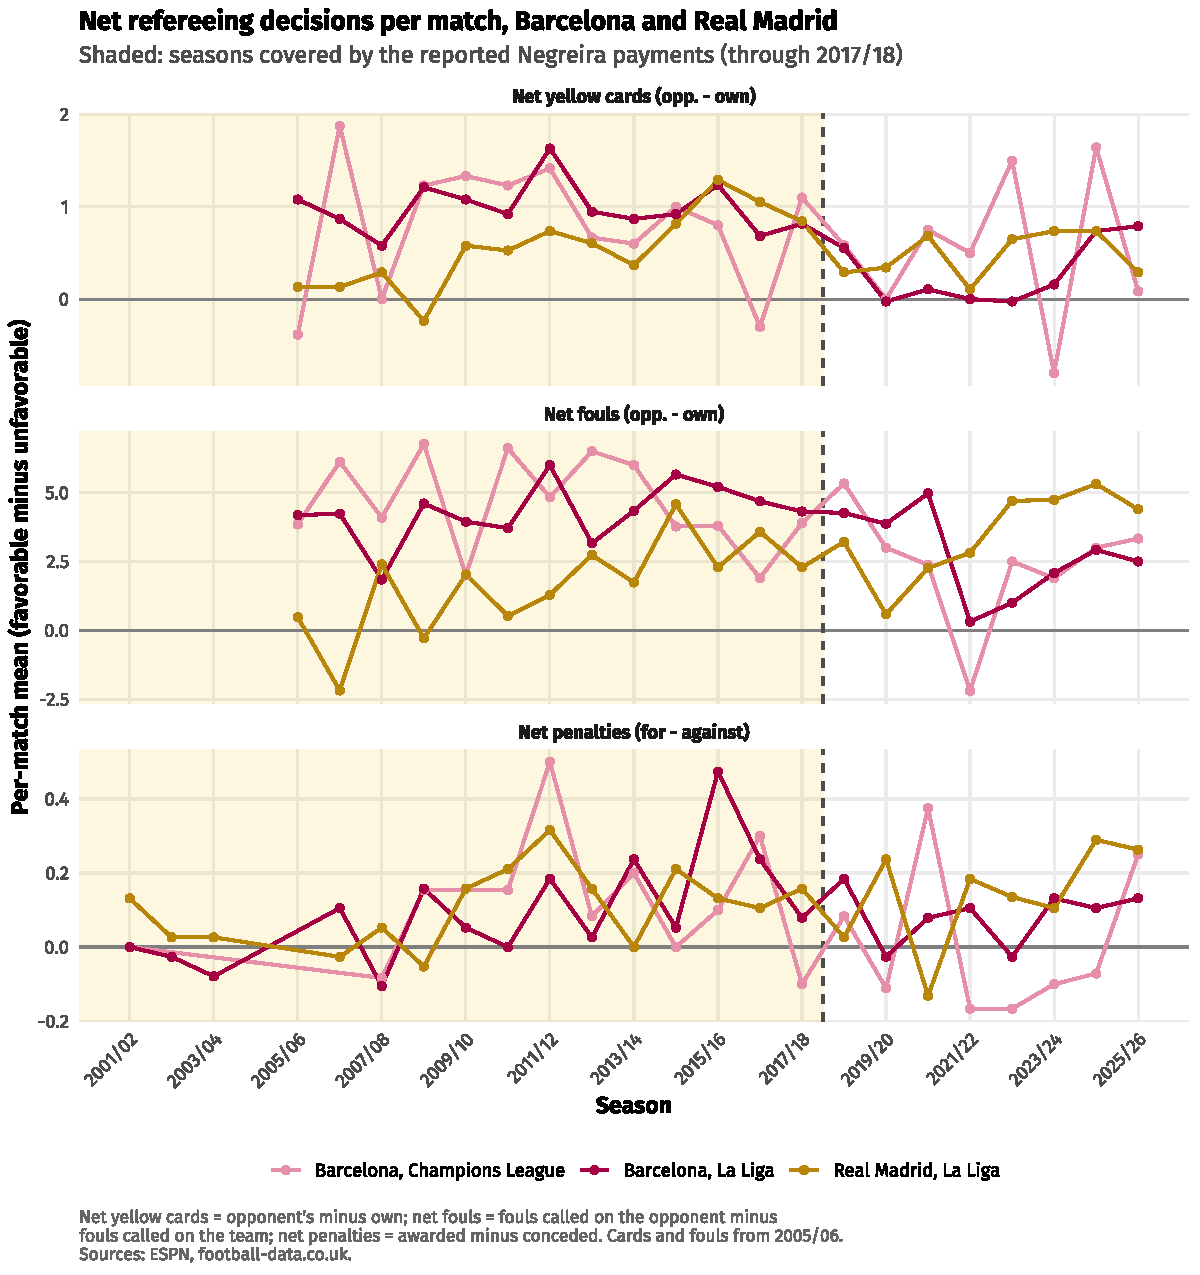
\includegraphics[width=\textwidth,height=0.8\textheight,keepaspectratio]{figure/figure-one-barcelona-raw-differentials.pdf}
\end{figure}
\clearpage

\begin{figure}[H]
  \centering
  \caption{Club Favorability Fixed Effects, Domestic Leagues \label{fig:ranks}}
  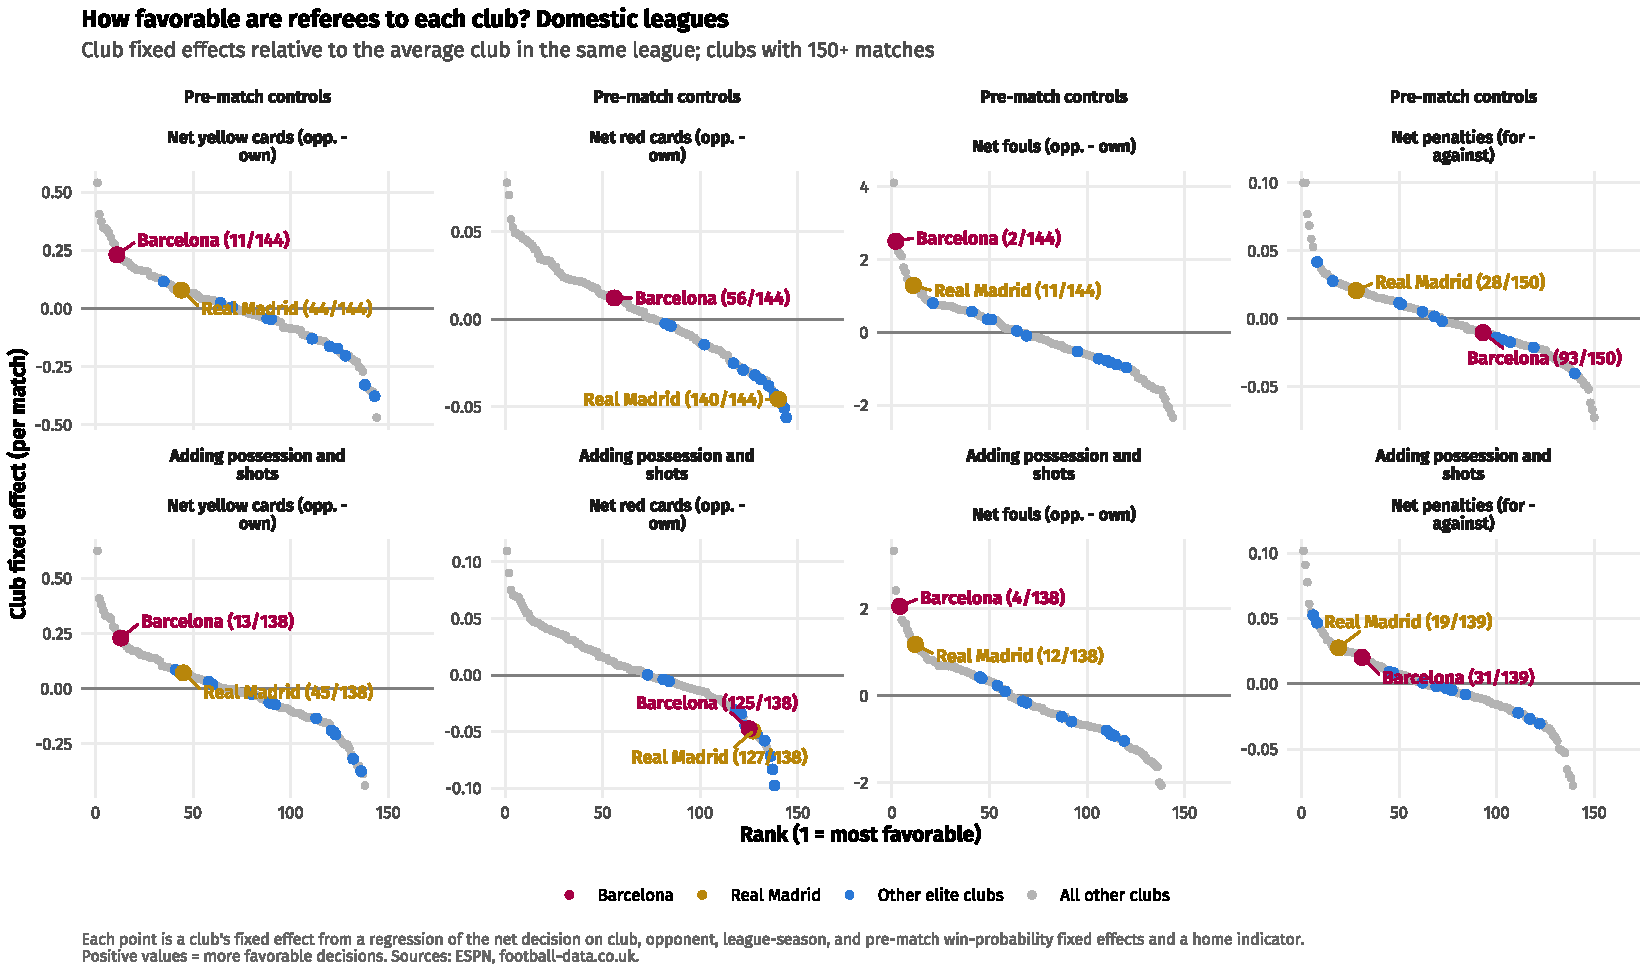
\includegraphics[width=\textwidth,height=0.8\textheight,keepaspectratio]{figure/figure-two-team-favorability-ranking.pdf}
\end{figure}
\clearpage

\begin{figure}[H]
  \centering
  \caption{Barcelona and Real Madrid Relative to the Average La Liga Club, by Season \label{fig:es}}
  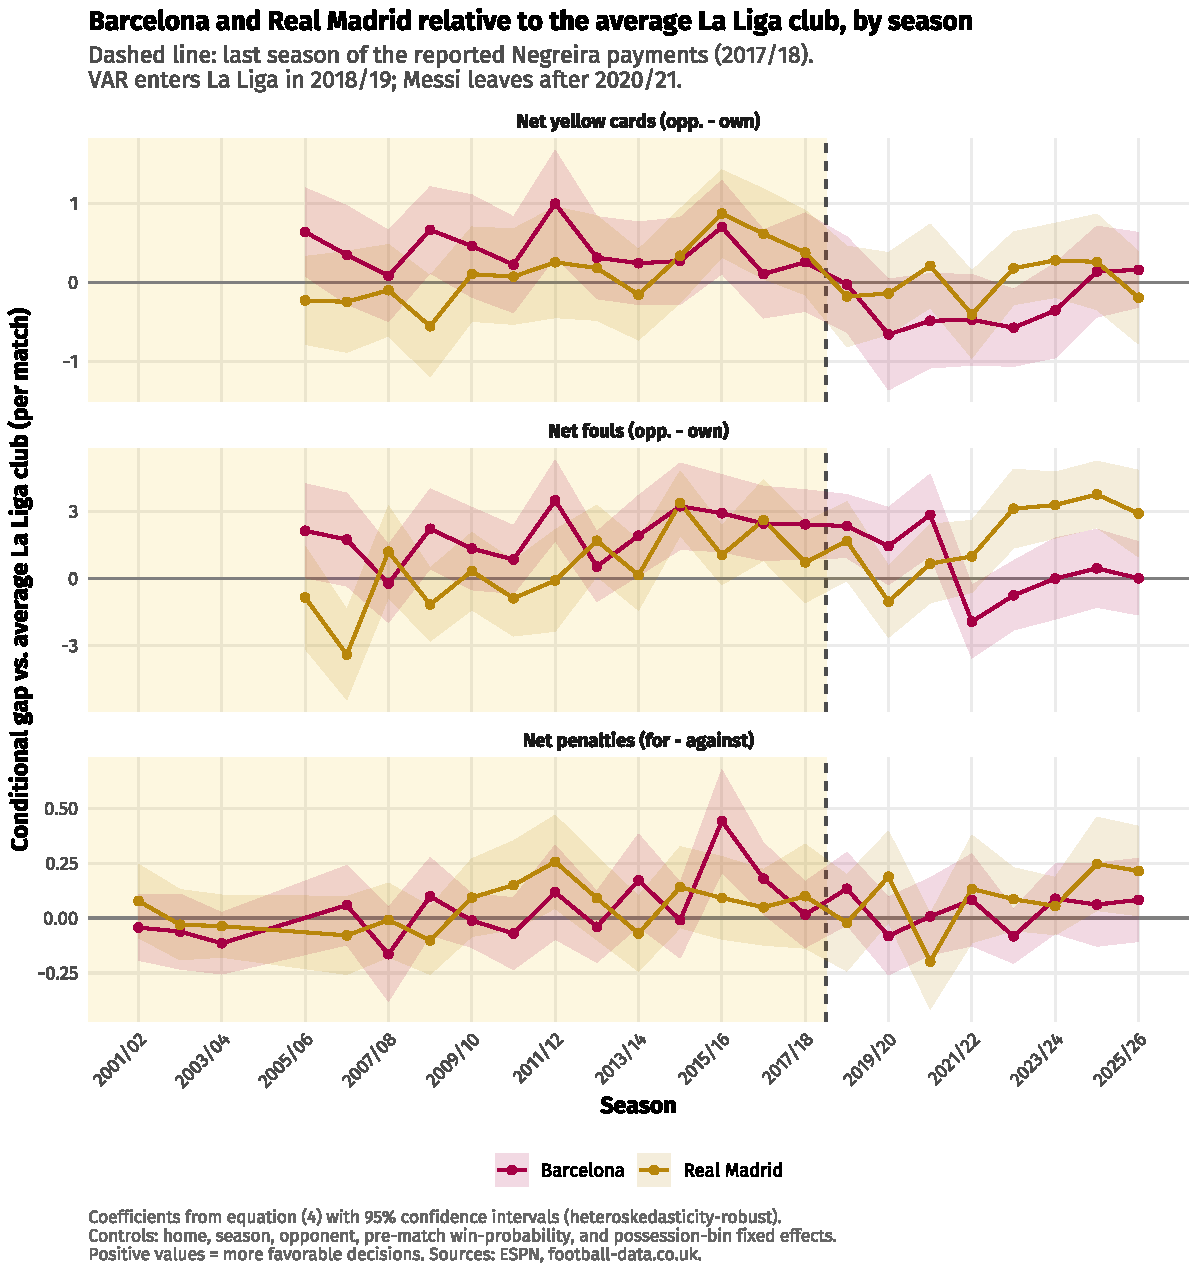
\includegraphics[width=\textwidth,height=0.8\textheight,keepaspectratio]{figure/figure-three-negreira-event-study.pdf}
\end{figure}

\begin{figure}[H]
  \centering
  \caption{Net Yellow Cards by Season: Barcelona and Real Madrid versus Europe's Elite Clubs \label{fig:elite-yellow}}
  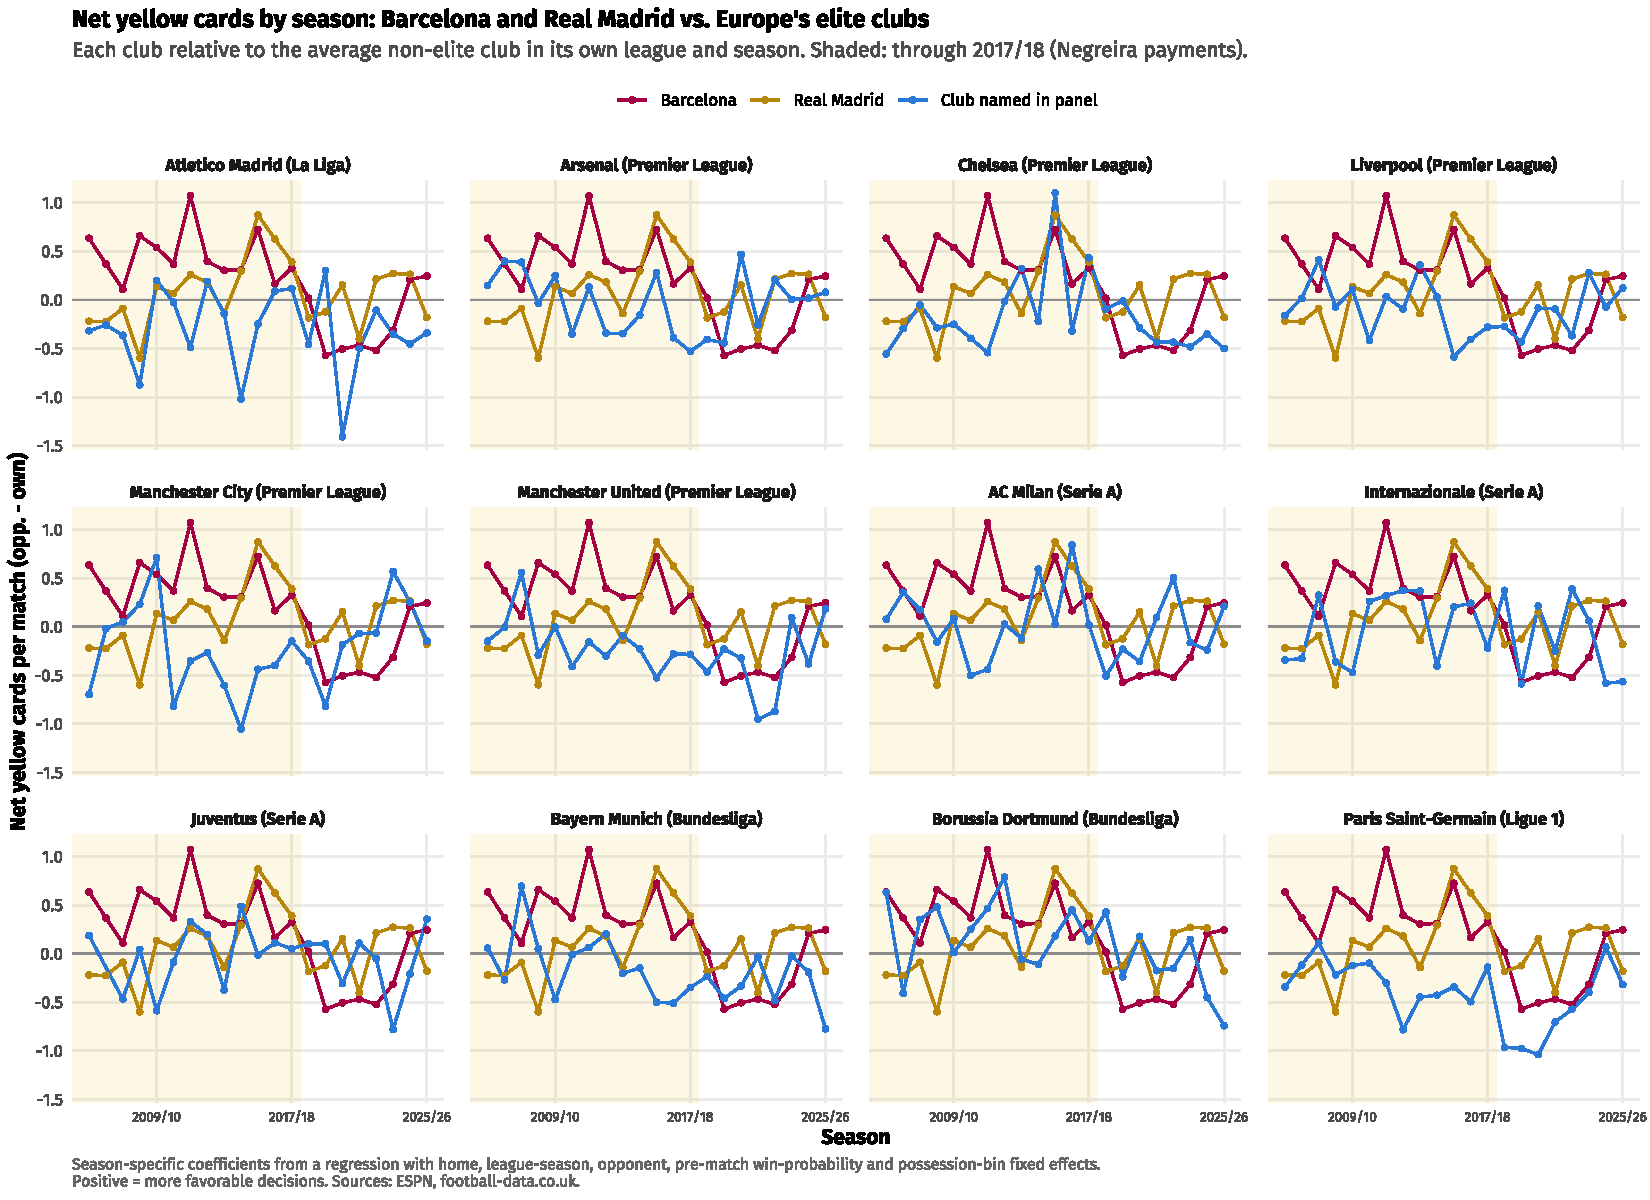
\includegraphics[width=\textwidth,height=0.8\textheight,keepaspectratio]{figure/figure-four-elite-net-yellow-by-season.pdf}
\end{figure}
\clearpage

\begin{figure}[H]
  \centering
  \caption{Net Fouls by Season: Barcelona and Real Madrid versus Europe's Elite Clubs \label{fig:elite-fouls}}
  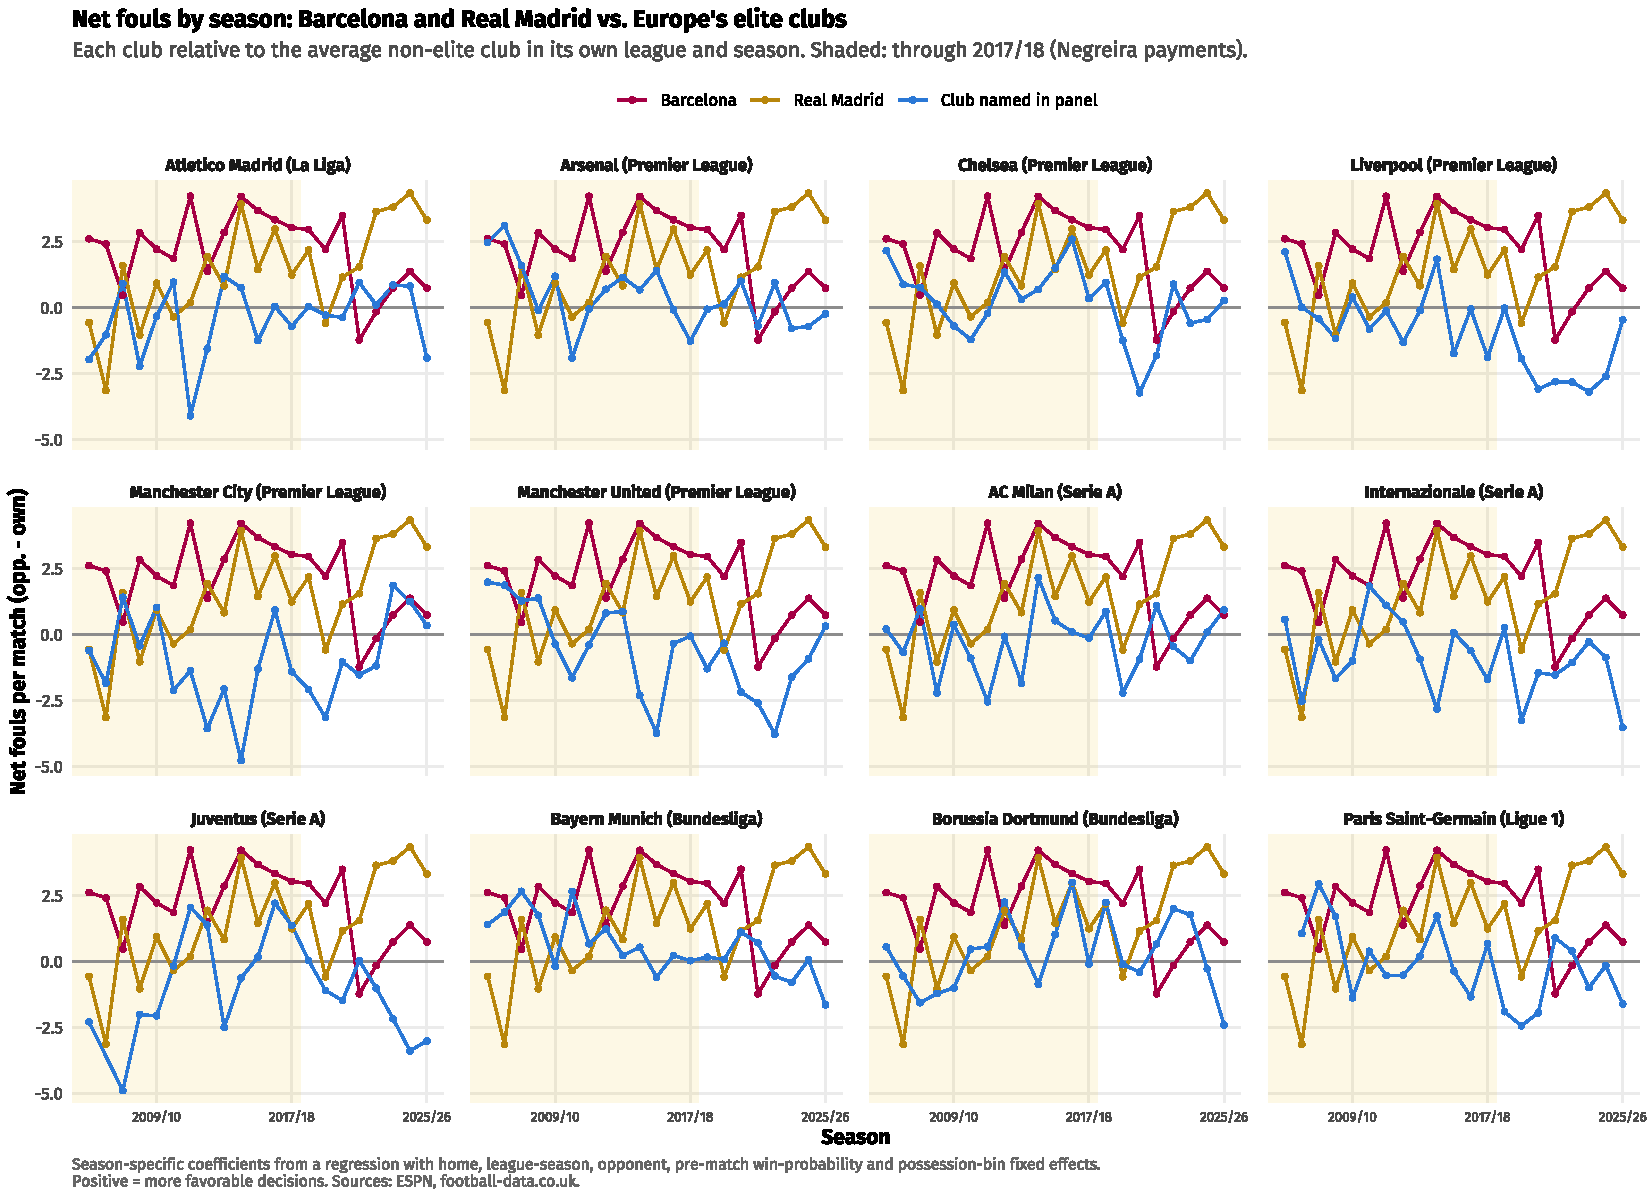
\includegraphics[width=\textwidth,height=0.8\textheight,keepaspectratio]{figure/figure-five-elite-net-fouls-by-season.pdf}
\end{figure}
\clearpage

\begin{figure}[H]
  \centering
  \caption{Net Penalties by Season: Barcelona and Real Madrid versus Europe's Elite Clubs \label{fig:elite-pens}}
  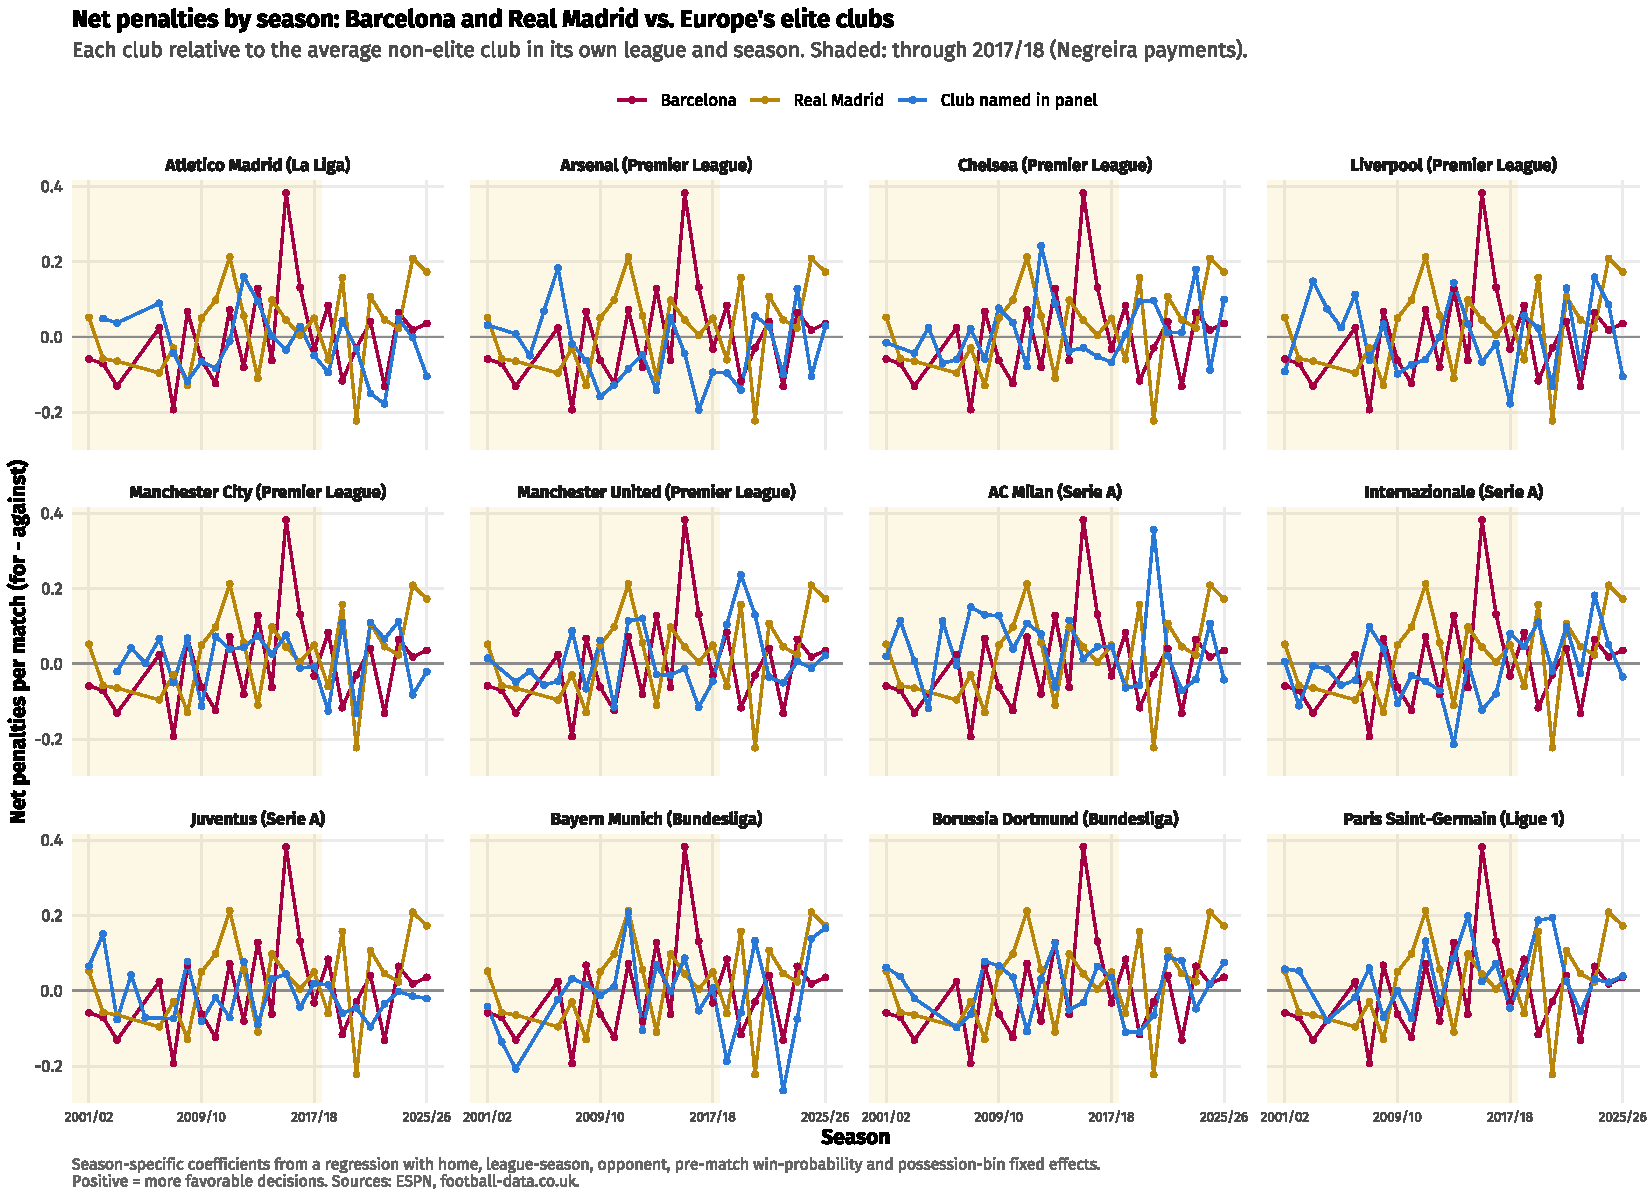
\includegraphics[width=\textwidth,height=0.8\textheight,keepaspectratio]{figure/figure-six-elite-net-penalties-by-season.pdf}
\end{figure}
\clearpage

\begin{figure}[H]
  \centering
  \caption{Refereeing Gaps by Club and Season \label{fig:elite-heatmap}}
  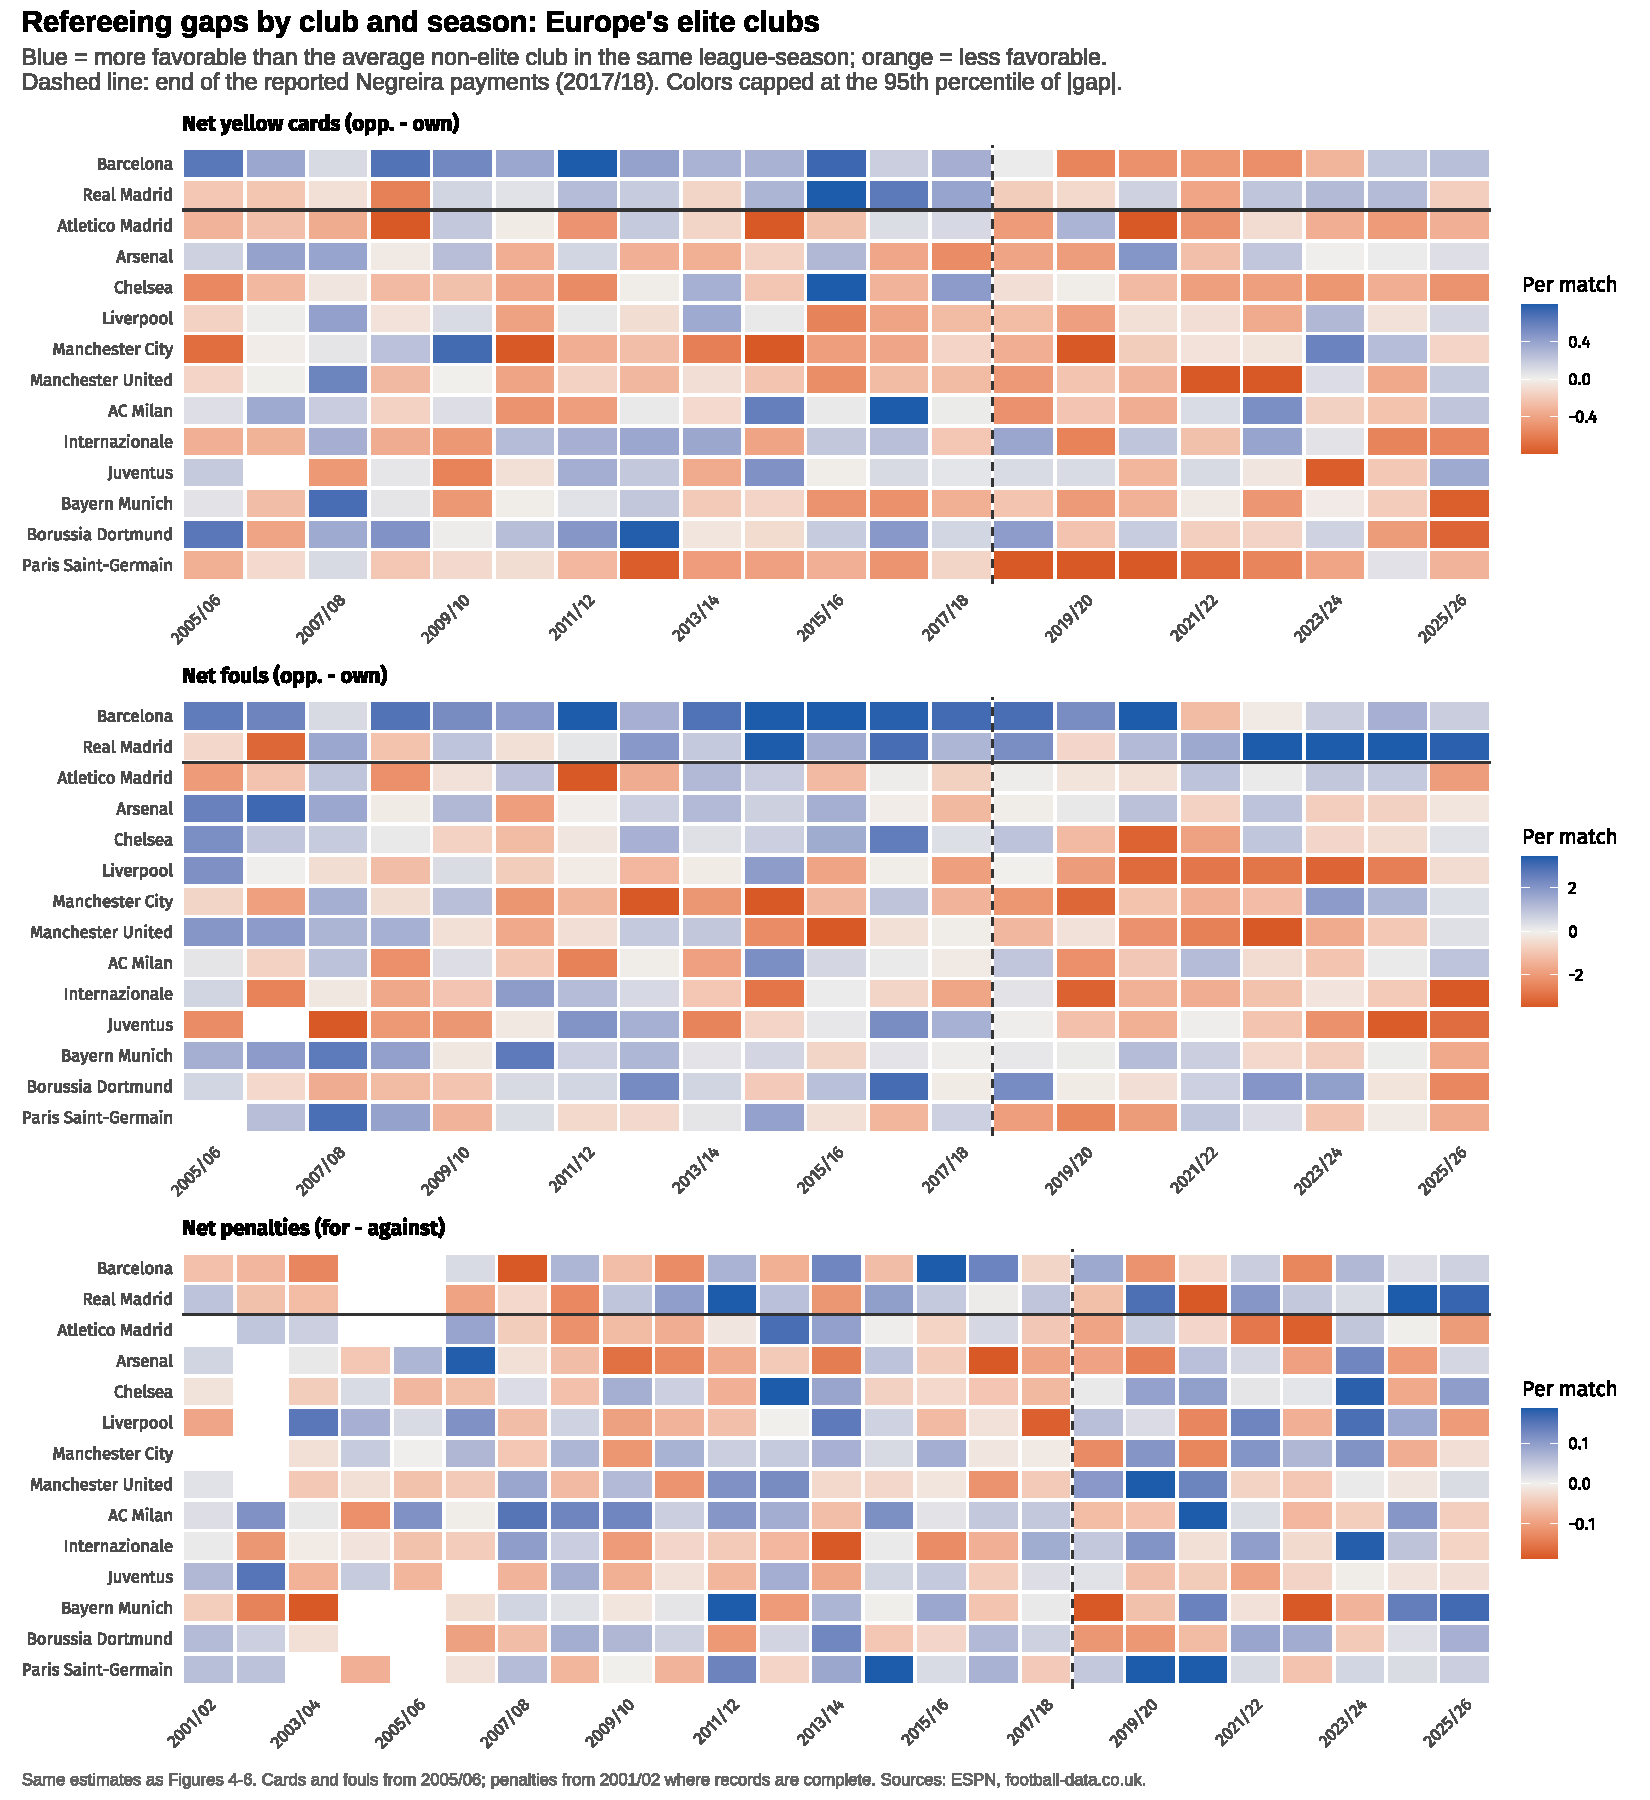
\includegraphics[width=\textwidth,height=0.85\textheight,keepaspectratio]{figure/figure-seven-elite-heatmap.pdf}
\end{figure}

\clearpage

\begin{figure}[H]
  \centering
  \caption{Real Madrid in the Champions League: Refereeing Gaps by Season \label{fig:rmucl}}
  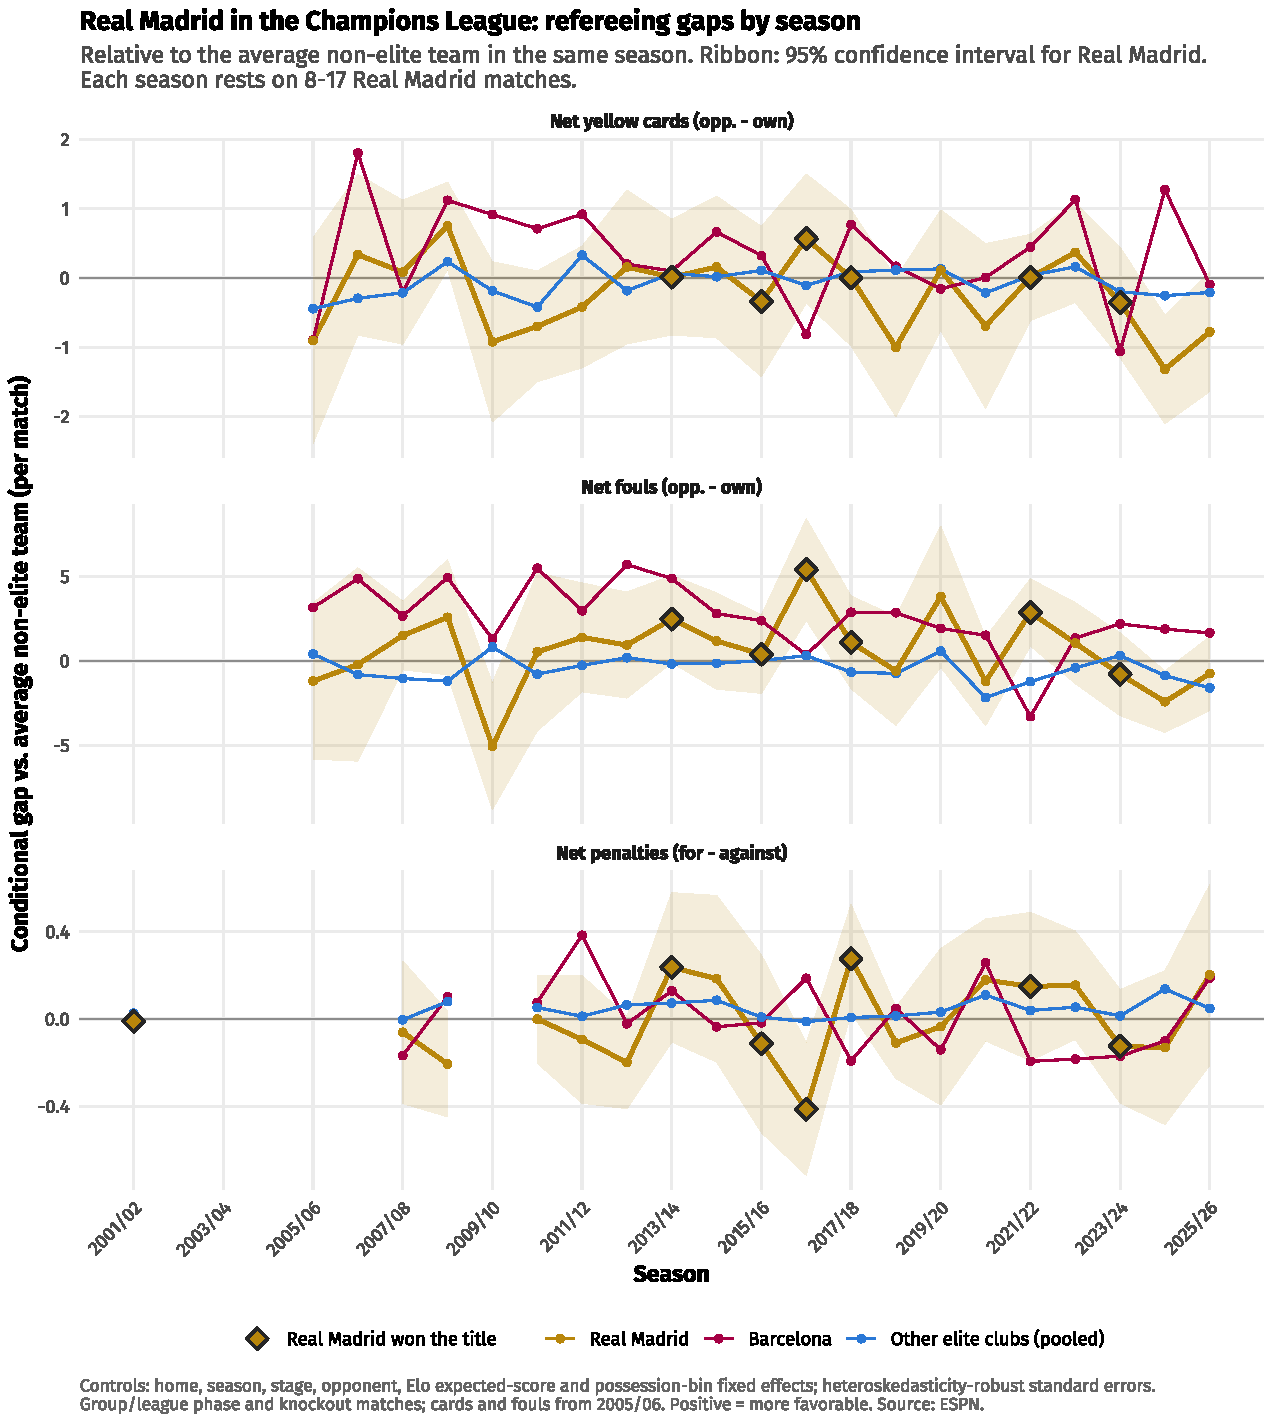
\includegraphics[width=\textwidth,height=0.85\textheight,keepaspectratio]{figure/figure-eight-real-madrid-champions-league-by-season.pdf}
\end{figure}

\end{document}
